\documentclass[11pt,a4paper]{amsart}
\usepackage[T1]{fontenc}
\usepackage{lmodern,microtype}
\usepackage[margin=29mm,headheight=14pt]{geometry}
\usepackage{amsmath,amssymb,mathtools,bm,mathrsfs,booktabs,array,enumitem}
\usepackage{xcolor,tikz}
\usetikzlibrary{arrows.meta,positioning,calc}
\usepackage[colorlinks=true,linkcolor=blue!45!black,citecolor=blue!45!black,urlcolor=blue!45!black]{hyperref}
\hypersetup{pdftitle={Twelve-Mode Ensemble Control of Navier--Stokes and Resistive MHD},pdfauthor={Harjas Sandhu}}
\setlength{\emergencystretch}{1.5em}
\setlist[enumerate]{leftmargin=*,itemsep=3pt,topsep=5pt}
\setlist[itemize]{leftmargin=*,itemsep=3pt,topsep=5pt}
\newtheorem{theorem}{Theorem}[section]
\newtheorem{proposition}[theorem]{Proposition}
\newtheorem{lemma}[theorem]{Lemma}
\newtheorem{corollary}[theorem]{Corollary}
\theoremstyle{definition}
\newtheorem{definition}[theorem]{Definition}
\newtheorem{example}[theorem]{Example}
\theoremstyle{remark}
\newtheorem{remark}[theorem]{Remark}
\numberwithin{equation}{section}
\newcommand{\T}{\mathbb T}
\newcommand{\R}{\mathbb R}
\newcommand{\Z}{\mathbb Z}
\newcommand{\N}{\mathbb N}
\newcommand{\Q}{\mathbb Q}
\newcommand{\PP}{\mathbb P}
\newcommand{\Bcal}{\mathcal B}
\newcommand{\Bhat}{\widehat{\Bcal}}
\newcommand{\Ccal}{\mathcal C}
\newcommand{\Mcal}{\mathcal M}
\newcommand{\Hcal}{\mathcal H}
\newcommand{\Ecal}{\mathcal E}
\newcommand{\Lc}{L}
\newcommand{\Cc}{C}
\newcommand{\ip}[2]{\langle #1,#2\rangle}
\newcommand{\norm}[1]{\lVert #1\rVert}
\newcommand{\abs}[1]{\lvert #1\rvert}
\newcommand{\mean}[1]{\langle #1\rangle}
\newcommand{\diver}{\operatorname{div}}
\newcommand{\curl}{\operatorname{curl}}
\newcommand{\supp}{\operatorname{supp}}
\newcommand{\Flow}{\operatorname{Fl}}
\newcommand{\esssup}{\operatorname*{ess\,sup}}
\newcommand{\push}[1]{(#1)_*}
\DeclareMathOperator{\Id}{Id}
\DeclareMathOperator{\Sym}{Sym}
\DeclareMathOperator{\Rea}{Re}
\DeclareMathOperator{\Ima}{Im}
\title[Twelve-mode ensemble control of fluids]{Twelve-Mode Ensemble Control\\ of Navier--Stokes and Resistive MHD}
\author{Harjas Sandhu}
\address{The University of Queensland}
\email{harjas.sandhu@student.uq.edu.au}
\date{11 November 2026}
\subjclass[2020]{35Q30, 35Q35, 35Q60, 93B05, 93C73}
\keywords{Navier--Stokes equations, resistive magnetohydrodynamics, ensemble control, finite-dimensional forcing, non-autonomous parabolic evolution}
\begin{document}
\begin{abstract}
We construct a single prescribed momentum force for an uncertainty class of three-dimensional viscous, resistive magnetohydrodynamic equations on the unit torus. The viscosity and magnetic diffusivity are unknown independent Lipschitz functions, with supplied positive lower bounds and a supplied temporal Lipschitz bound. For every unknown initial pair in a joint $H^1$ ball, the same force prepares a chosen finite Fourier velocity target and returns the magnetic field close to its own unknown conserved mean. The conclusion holds for every admitted additive disturbance and every energy-admissible Leray--Hopf realization. The force uses exactly the twelve fundamental shear fields and ordinary rational time polynomials of degree at most four. A deterministic compiler has fixed polynomial numerical and complete binary resource bounds. The proof combines a concrete returning pressure-driven reset, coupled energy estimates, a full-space nonidentical-cell heat comparison and a depth-two target writer. Navier--Stokes and constant-coefficient cases are specializations. The results concern costly finite-time endpoints with globally supported periodic forcing, not path tracking, zero diffusivity or an economical physical actuator realization.
\end{abstract}
\maketitle

% ---- sections/01-introduction ----
\section{Introduction}\label{sec:introduction}
A force chosen after the initial state and the transport coefficients are known solves a different problem from a force prescribed before either is available. The distinction is particularly sharp for a conducting fluid. Mechanical stirring can increase magnetic diffusion, but it also stretches the magnetic field; the resulting Lorentz force changes the velocity that produced the stirring. Unknown coefficients affect both processes. A useful common control must close these effects in the physical coupled equations.

This paper constructs such a control on the periodic three-dimensional domain. One ordinary additive momentum force, using twelve fixed Fourier fields, first erases the unknown velocity and magnetic fluctuations, then writes a chosen velocity. It retains the unknown conserved magnetic mean. The same force works for an entire $H^1$ preparation ball, all admitted additive disturbances, and a continuum of independent time-dependent viscosity and resistivity profiles. The coefficient functions are Lipschitz with supplied bounds; their values are never measured or evaluated. The construction supplies a deterministic finite compiler and separate numerical and binary resource bounds.

The endpoint is deliberately asymmetric. Velocity is prescribed, whereas the magnetic target is its own unknown initial mean $H$. Mechanical forcing cannot create a nonzero magnetic field from zero magnetic input, nor can it change the periodic magnetic mean. The result controls the fluctuations in that invariant sector. It is not a theorem for arbitrary joint magnetic targets, and it uses neither a chosen magnetic source nor an additional imposed velocity. A separate companion \cite{SeedPreparation} prepares a nontrivial magnetic field from a supplied oriented seed, with calibrated viscosity for kinetic recovery. That preparation operation and the common eraser here have different initial-state contracts; neither construction is used as a premise for the other.

\subsection{The contribution}
The main result is Theorem~\ref{thm:main}. Its quantifier order is
\[
 (\hbox{bounds},V)\longmapsto(f,\eta),\qquad
 \forall(\nu(\cdot),\rho(\cdot)),\ \forall(u_0,B_0),\ \forall h,
 \ \forall\hbox{ admitted realizations}.
\]
The infinite-dimensional temporal uncertainty and the unknown harmonic magnetic field are included in this same common-input statement. The force consists of finitely many rational time polynomials, of degree at most four. Its numerical bounds are polynomial in inverse accuracies, inverse positive diffusivity bounds, preparation size, inverse time and the Lipschitz bound; they are not polynomial in binary input length alone.

Three mechanisms make this statement constructive. First, a concrete fourth-order shear word returns its entire transport geometry exactly while leaving a compact, modewise dissipative pressure effect in the physical Euler linearization. A fixed rational rotational design makes that effect dissipative on every mode and both polarizations. Exact transport return allows a bounded-operator Taylor remainder on the actual rough preparation spaces. Stable repetition is controlled by $ns^5$, while useful contraction accumulates on the distinct scale $ns^4$.

Second, the magnetic evolution is compared on the full solenoidal $H^1$ space with a product of commuting scalar heat maps. This comparison includes constants and permits nonidentical complete cells. Its operator error is bounded by
\[
 CG^8[(\ell/T)^{1/4}+\beta]+12G^2\Lambda_0\ell,
\]
where $G$ is a paid spatial and ellipticity envelope, $\ell$ is the largest cell length and $\beta$ is the reset fraction. A whole-macro form estimate avoids multiplying the freezing error by the number of cells. The residual harmonic bias and the nonlinear induction source are then controlled by one global convolution estimate, coupled to local Lorentz estimates and velocity resets.

Third, signed quadratic lowering reduces the fixed enlarged reset family to the twelve physical fields, while a separate depth-two polarization construction writes a variable Fourier target with polynomial conditioning. The proof retains ordinary forces, exact product-coordinate returns, continuous coefficient-dependent analysis correctors and complete rational precision costs. It does not replace any of these operations by an assumed saturation or stability package.

\subsection{Earlier control and parabolic machinery}
Finite-mode fluid control and quadratic saturation are established methods. Agrachev and Sarychev \cite{AS2005} developed control through low Fourier modes, including finite-dimensional Galerkin systems and infinite-dimensional two-dimensional conclusions. Shirikyan \cite{Shirikyan2006} extended the approach to approximate control of the three-dimensional Navier--Stokes equation. Nersesyan \cite[Theorem~2.2]{Nersesyan2015} obtains approximate control of velocity together with Lagrangian motion for fixed viscosity and prescribed data; his Theorem~4.1 and Proposition~4.3 give the relevant finite Fourier saturation algebra. We give the rational signed generation needed here explicitly. Neither twelve-mode saturation itself nor the quadratic convexification mechanism is claimed as new. The issue addressed here is a single quantitatively compiled force for unknown states and unknown coefficient functions, with the coupled magnetic error included.

MHD controllability also predates this work. Galan \cite[Theorem~2.1]{Galan2011} treats periodic distributed controls in both equations. Tao, Yao and Yin \cite{TYY2025} study local trajectory control by velocity forcing in two-dimensional bounded geometry. Liao, Sueur and Zhang \cite[Theorem~1.1]{LSZ2025} prove small-time approximate null control for a three-dimensional viscous non-resistive system through boundary control of both fields, with substantially smoother preparation assumptions. These are different control ports, geometries and uncertainty classes. Our theorem neither subsumes their results nor asserts first-ever MHD or velocity-only MHD control. The classical weak and strong solution theory is developed, for example, by Sermange and Temam \cite{ST1983}; the non-autonomous existence and transfer steps needed here are proved directly below.

For parabolic evolution we use the measurable bounded quasi-coercive form theorem of Lions, stated as Theorem~1.1 in Arendt, Dier, Laasri and Ouhabaz \cite{ADLO2014}. It gives variational evolution in the dual of the form domain. It does not give arbitrary maximal regularity in the pivot Hilbert space. Fackler's counterexamples \cite[Theorem~5.1]{Fackler2017} explain this distinction. Our spatial smoothing and adjoint bounds are derived for the actual scalar-principal vector diffusion operator, with fixed common spaces and without temporal derivatives of its fast geometry. The Bessel identities and fixed-order asymptotics used in target synthesis are classical \cite{DLMF}; the uniform conditioning estimate needed by the compiler is proved from them.

\subsection{Scope and organization}
The theorem concerns costly finite-time endpoints in an explicit periodic model with globally supported Fourier forcing. It keeps known positive lower diffusivity bounds, a supplied temporal Lipschitz bound and an $H^1$ preparation class. It proves strong continuation for the designed controls, then transfers the result to every energy-admissible weak realization. It is not an unforced global-regularity assertion. No economical authority bound, laboratory actuator implementation or exhaustive historical-priority claim is made.

Section~\ref{sec:setting} states the full contract. Section~\ref{sec:overview} explains the proof mechanism before the technical estimates. Sections~\ref{sec:foundations}--\ref{sec:reset} prove the concrete reset and its coupled physical realization. Sections~\ref{sec:stirring}--\ref{sec:parabolic} construct the common magnetic eraser. Section~\ref{sec:compiler} supplies lowering and target writing; Section~\ref{sec:schedule} closes the common schedule and resource calculation. Section~\ref{sec:weak} proves the all-realization statement. The appendices provide finite arithmetic and analytic details needed to reproduce the estimates.



% ---- sections/02-setting ----
\section{The equation, the uncertainty class and the main result}\label{sec:setting}
Let $\T^3=\R^3/\Z^3$ have volume one, and put $\kappa=2\pi$. We use real vector fields, allowing complex Fourier notation in proofs. The periodic Leray projection $P$ has symbol
\[
 P_k=I-\frac{k\otimes k}{|k|^2}\quad(k\ne0),\qquad P_0=I.
\]
Thus constants are included. For solenoidal fields set
\[
 \Bcal(v,z)=P((v\cdot\nabla)z),\quad
 L_vz=\Bcal(v,z)+\Bcal(z,v),\quad
 C_vz=(v\cdot\nabla)z-(z\cdot\nabla)v.
\]
The full Sobolev norm is
\begin{equation}\label{eq:Hs}
 \norm v_{H^s}^2=\sum_{k\in\Z^3}(1+\kappa^2|k|^2)^s|\widehat v(k)|^2,
 \qquad
 \norm{(v,b)}_{\Hcal^s}^2=\norm v_{H^s}^2+\norm b_{H^s}^2.
\end{equation}
In particular $\norm H_{H^s}=|H|$ for a constant field. A subscript zero means zero spatial mean. The symbol $J$ denotes $I-\Delta$; the weight $J^{-1/2}$ parametrizes the $H^1$ ball isometrically from $L^2$ and is compact as an $L^2$ operator.

We consider
\begin{equation}\label{eq:mhd}
 \begin{aligned}
 u_t&=\nu(t)\Delta u-\Bcal(u,u)+\Bcal(B,B)+f+h_u,\\
 B_t&=\rho(t)\Delta B-C_uB+h_B,\\
 \diver u&=\diver B=0,\qquad \mean u=0.
 \end{aligned}
\end{equation}
All chosen forces belong to the same space
\begin{equation}\label{eq:twelve}
 \Ecal=\operatorname{span}_{\R}\{e_i\cos(\kappa x_j),\ e_i\sin(\kappa x_j):1\le i,j\le3,\ i\ne j\}.
\end{equation}
It has dimension twelve. There is no chosen source in the induction equation.
The disturbance is a measurable solenoidal, mean-zero pair $h=(h_u,h_B)$, bounded in $L^\infty(0,\tau;\Hcal^0)$. Integrating the induction equation gives
\begin{equation}\label{eq:mean}
 \mean{B(t)}=\mean{B_0}=:H.
\end{equation}
Neither $H$ nor any description of $B_0$ is supplied to the control program.

\begin{definition}[Admitted realization]\label{def:weak}
An admitted realization of \eqref{eq:mhd} is a solenoidal pair in
$L^\infty(0,\tau;\Hcal^0)\cap L^2(0,\tau;\Hcal^1)$, weakly continuous into $\Hcal^0$ on $[0,\tau]$, satisfying the distributional equations, the given initial data, and the total-energy inequality
\begin{align}\label{eq:energy}
 \frac12\norm{(u,B)(t)}_2^2
 &+\int_s^t\bigl(\nu(r)\norm{\nabla u(r)}_2^2+
                 \rho(r)\norm{\nabla B(r)}_2^2\bigr)\,dr\notag\\
 &\le\frac12\norm{(u,B)(s)}_2^2+
 \int_s^t\bigl[\ip{f+h_u}{u}+\ip{h_B}{B}\bigr]\,dr
\end{align}
for $s=0$ and almost every $s>0$, and every later energy trace $t$. At $t=\tau$ use the weak left trace, with its norm bounded by the lower limit of the preceding energies. Equivalently one may include this one-sided inequality in the admissible endpoint convention. The controlled strong solution constructed below is continuous in $\Hcal^1$, so all these conventions give the same terminal field for this construction.
\end{definition}

\begin{theorem}[Common finite-mode reset and write]\label{thm:main}
There exist fixed effectively computable integers $A,p\ge1$ and a total deterministic compiler with the following property. Its input consists of binary rationals
\[
 M\ge1,\quad 0<\nu_-\le\nu_+\le1,\quad
 0<\rho_-\le\rho_+\le1,\quad
 0<\tau\le1,\quad0<\epsilon<1,\quad\Lambda\ge1,
\]
and a real, mean-zero solenoidal rational finite Fourier polynomial $V$, promised to satisfy $\norm V_{H^1}\le M$. The complete variable list of integer frequencies, rational coefficients and polarizations, with their denominators, is part of the input. Let $L$ be its complete binary length, and set
\begin{equation}\label{eq:R}
 R=2+M+\nu_-^{-1}+\rho_-^{-1}+\tau^{-1}+\epsilon^{-1}+\Lambda.
\end{equation}
The output is a positive rational $\eta$ and one finite rational partition of $[0,\tau]$, with ordinary rational polynomial coefficients of degree at most four for a force $f(t)\in\Ecal$ on every partition interval.

For every pair of real functions $\nu,\rho$ with values in the supplied intervals and individual Lipschitz constants at most $\Lambda$, every unknown real solenoidal initial pair with $\mean{u_0}=0$ and $\norm{(u_0,B_0)}_{\Hcal^1}\le M$, every admitted disturbance with
$\esssup_t\norm{h(t)}_{\Hcal^0}\le\eta$, and every admitted realization, the \emph{same} output satisfies
\begin{equation}\label{eq:endpoint}
 \left(\norm{u(\tau)-V}_2^2+\norm{B(\tau)-H}_2^2\right)^{1/2}
 \le\epsilon,\qquad H=\mean{B_0}.
\end{equation}
It also satisfies
\begin{equation}\label{eq:physical}
 \eta^{-1},\quad \sup_{0\le t\le\tau}\norm{f(t)}_{W^{1,\infty}},\quad
 \int_0^\tau\norm{f(t)}_{W^{1,\infty}}\,dt\le AR^p.
\end{equation}
Bit operations, memory bits, total output bits, interval count, polynomial degrees and individual rational bit lengths are at most $A(L+R)^p$. The constants are independent of the target catalogue, all actual coefficient functions, the magnetic mean, initial fields, disturbances and realizations. Values, derivatives, samples and descriptions of the actual coefficient functions are never compiler inputs.
\end{theorem}

The numerical parameter $R$ contains inverse accuracies and inverse diffusivities. The theorem is not a polynomial-time assertion in binary input length alone. The finite precomputation defining the universal constants is part of the cost, even though it is not necessary to execute that enormous precomputation to prove its termination.

\begin{corollary}[Navier--Stokes and constant-parameter special cases]\label{cor:NS}
With $B_0=h_B=0$, the same construction gives a common all-realization velocity endpoint theorem for Navier--Stokes with unknown Lipschitz viscosity. Constant unknown viscosity and resistivity, known positive coefficients, and prescribed known conserved flux are special cases. These conclusions use independently proved reset and synthesis lemmas below; the Navier--Stokes specialization is not used to justify its own foundations.
\end{corollary}
\begin{proof}
The field $B=0$ is a solution of the induction equation when $B_0=h_B=0$. The strong-solution comparison proved in Section~\ref{sec:weak} makes it the magnetic component of every admitted controlled realization. Restricting the coefficient and initial-state uncertainty sets gives the other cases.
\end{proof}



% ---- sections/03-overview ----
\section{Conceptual overview and a small cancellation example}\label{sec:overview}
The control is an open-loop program. Its initial reset brings velocity to a small prescribed radius without learning the initial state. Repeated stirring cells then dissipate magnetic fluctuations while further resets suppress Lorentz-generated velocity. A wait uses the unused time, and a finite writer produces the target velocity at the exact endpoint.

\begin{center}
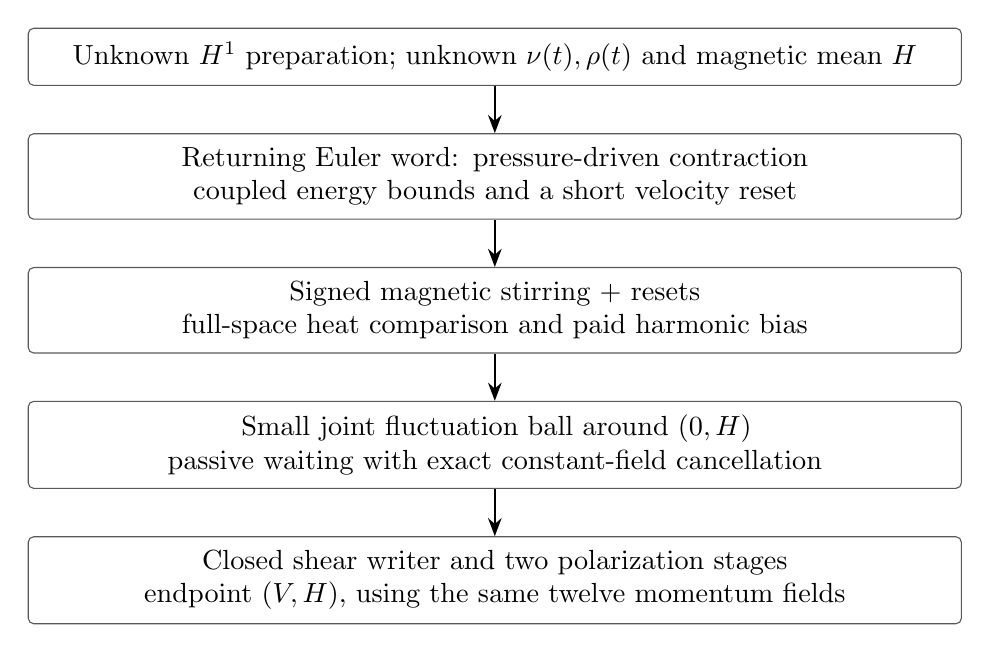
\begin{tikzpicture}[node distance=6mm,box/.style={draw=black!65,rounded corners=2pt,align=center,text width=11.5cm,inner sep=5pt},arr/.style={-{Stealth[length=2.3mm]},thick}]
\node[box] (a) {Unknown $H^1$ preparation; unknown $\nu(t),\rho(t)$ and magnetic mean $H$};
\node[box,below=of a] (b) {Returning Euler word: pressure-driven contraction\\ coupled energy bounds and a short velocity reset};
\node[box,below=of b] (c) {Signed magnetic stirring $+$ resets\\ full-space heat comparison and paid harmonic bias};
\node[box,below=of c] (d) {Small joint fluctuation ball around $(0,H)$\\ passive waiting with exact constant-field cancellation};
\node[box,below=of d] (e) {Closed shear writer and two polarization stages\\ endpoint $(V,H)$, using the same twelve momentum fields};
\draw[arr] (a)--(b);\draw[arr] (b)--(c);\draw[arr] (c)--(d);\draw[arr] (d)--(e);
\end{tikzpicture}
\end{center}

There are two different homogeneous maps. The velocity perturbation is propagated by the physical linearized Euler operator $L_w$, including the Leray pressure and strain. A magnetic field is transported by the Lie derivative $C_w$ and hence by vector pushforward. A closed particle-motion word can have nontrivial velocity action while its magnetic pushforward returns exactly to identity. Treating these maps as the same would remove the mechanism of the reset.

\begin{example}[Why temporal uncertainty needs a paid cancellation]\label{ex:affine}
For one shear $F$ and a constant analysis viscosity, the exact affine action of an impulse $a$ is
\[
 \mathcal A_F^\nu(a)z=Q_F(a)z+\nu a\Delta F,
 \qquad Q_F(a)\Delta F=\Delta F.
\]
Thus $\mathcal A_F^\nu(a)\mathcal A_F^\nu(-a)=I$. If the two legs instead have unrelated viscosities $\nu_1,\nu_2$, their composition is
\[
 z\longmapsto z+(\nu_2-\nu_1)a\Delta F.
\]
Shortening the legs alone does not reduce this residue. With a supplied Lipschitz bound, two values within a complete word differ by at most its duration times that bound. The additional error can then be paid by a polynomial time refinement. All frozen values in this reasoning belong to the proof; none is sampled by the program.
\end{example}

Likewise, short diffusion is not uniformly close to identity on an $H^1$ ball: high Fourier modes remain sensitive at every positive time. The proof uses its coercive energy and smoothing instead. The full-space comparison also pays the fluctuation generated from a constant magnetic input; a mean-zero contraction estimate alone would miss that term.



% ---- sections/04-foundations ----
\section{A physical reset word and its uniform estimates}
\label{fnd:section}\label{sec:foundations}

The reset acts on the complete three-dimensional velocity linearization,
including stretching. Its mechanism is an exact transport return with a nonzero
fourth-order pressure effect. This permits bounded-operator estimates on Sobolev
balls, although individual transport operators are not close to the identity in
those operator norms.

Use $\kappa,P,\Bcal,L_F$ and the Sobolev norms defined in Section~\ref{sec:setting}. 

\subsection{An exact return of the transport geometry}

For invertible operators set $\mathcal C(A,B)=ABA^{-1}B^{-1}$ and define
\begin{align}
 H_2(s;X,Y)&=\mathcal C(e^{sX},e^{sY}),\notag\\
 H_3(s;X,Y)&=\mathcal C(e^{sY},H_2(s;X,Y)),\notag\\
 H_4(s;X,Y)&=\mathcal C(e^{sX},H_3(s;X,Y)).
 \label{fnd:words}
\end{align}
The words have $4,10,22$ exponential letters, respectively. Multiplication of
the noncommutative Taylor polynomials through degree four gives
\begin{equation}
 H_4(s;X,Y)=I+s^4[X,[Y,[X,Y]]]+O(s^5)
 \label{fnd:formal-word}
\end{equation}
on smooth vectors. We justify the remainder in actual operator norm below.

\begin{lemma}[Complete transport return]\label{fnd:transport-return}
Let $i,j,\ell$ be distinct, $F=e_i f(x_j)$, and $G=e_j g(x_\ell)$.
The underlying vector-pushforward transport map of
$H_4(s;L_F/2,L_G)$ is exactly the identity for every real $s$.
The same holds after a common rotation and spatial dilation and for the inverse
word.
\end{lemma}
\begin{proof}
In coordinates $(x,y,z)=(x_i,x_j,x_\ell)$, the elementary flows are
\[
 A_\alpha(x,y,z)=(x+\alpha f(y),y,z),\qquad
 B_\beta(x,y,z)=(x,y+\beta g(z),z).
\]
Their group commutator is
\[
 A_\alpha B_\beta A_\alpha^{-1}B_\beta^{-1}(x,y,z)
 =\bigl(x+\alpha[f(y)-f(y-\beta g(z))],y,z\bigr).
\]
It is an $x$-shear depending only on $(y,z)$. Its commutator with $B_\beta$ has
the same form. All such $x$-shears commute with $A_\alpha$, so the final
commutator is exactly the identity. The sign convention relating $e^{tL_F}$
to the flow of $F$ merely changes $\alpha,\beta$. Common rotations and dilations
preserve this identity, as does inversion.
\end{proof}

\subsection{The fourth-order Fourier symbol}

Let $A_{ij}^{c}=L_{e_i\cos(\kappa x_j)}$ and
$A_{ij}^{s}=L_{e_i\sin(\kappa x_j)}$. Define
\begin{align}
 Z(A,B)&=[A,[B,[A,B]]]=2ABAB-2BABA-A^2B^2+B^2A^2,\notag\\
 D_4&=\frac14\sum_{i,j,\ell\ {\rm distinct}}
       \sum_{\alpha,\beta\in\{c,s\}}
       Z(A_{ij}^{\alpha},A_{j\ell}^{\beta}).
 \label{fnd:D4}
\end{align}
Concatenate $H_4(s;A_{ij}^{\alpha}/2,A_{j\ell}^{\beta})$ over its $24$
summands. The result has $528$ letters. Every letter is a genuine physical
linearized shear evolution with signed impulse $\pm s$ or $\pm s/2$.

For a transition $k\mapsto k+\sigma e_j$ put
\begin{equation}
 T_{ij,\sigma}(k)=P_{k+\sigma e_j}
          (k_iI+\sigma e_ie_j^{\mathsf T})P_k.
 \label{fnd:transition}
\end{equation}
Its cosine coefficient is $i\kappa T_{ij,\sigma}(k)/2$. Each degree-four
monomial has two shifts in each of directions $j,\ell$. The cosine--sine sum
cancels the equal-sign pairs. Thus $D_4$ is exactly Fourier diagonal. Write
$D_4(k)=\kappa^4d(k)$; retaining every intermediate projection gives
\begin{equation}
 d(k)=\frac1{16}\sum_{i,j,\ell\ {\rm distinct}}
       \sum_{\sigma,\rho=\pm1}
       (2ABAB-2BABA-AABB+BBAA)(k).
 \label{fnd:d-symbol}
\end{equation}
Here each $A$ is its transition in direction $e_j$, its two shifts have opposite
signs, and similarly for $B$ in direction $e_\ell$. Products act from right to
left. The formula also defines the symbol for real $k\ne0$, with the removable
resonances interpreted below. The unaveraged operator is not globally
dissipative: $d(e_1)|_{e_1^\perp}=-I/3$, but the two transverse eigenvalues at
$e_1+e_2$ are $1/45$ and $8/45$.

\begin{lemma}[Resonance modulus]\label{fnd:resonance}
The full matrix $d(k)$ is locally Lipschitz on $\mathbb R^3\setminus\{0\}$,
including every intermediate zero-frequency resonance. For $r=|k|>0$,
\begin{align}
 \|d(k)\|&\le2304(r+2)^4,\notag\\
 \|\nabla d(k)\|&\le18432(r+2)^3+4608(r+2)^4/r
 \quad\hbox{almost everywhere}.
 \label{fnd:modulus}
\end{align}
\end{lemma}
\begin{proof}
Put $Q_i(p)=p_iI+e_ip^{\mathsf T}-2p_i pp^{\mathsf T}/|p|^2$ for $p\ne0$,
and $Q_i(0)=0$. Then $p^{\mathsf T}Q_i(p)=0$, $\|Q_i(p)\|\le4|p|$, and
$Q_i$ is globally $8$-Lipschitz. Indeed, the derivative of
$p_i pp^{\mathsf T}/|p|^2$ has norm at most $3$; the other terms contribute at
most $2$. Homogeneity and continuity extend the estimate across zero.
For $p=k+\sigma e_j$, incompressibility gives exactly
$T_{ij,\sigma}(k)=Q_i(p)P_k$. Since $Q_i(p)$ already has range in $p^\perp$,
all internal $P_p$ can be removed. A returning path is therefore
$Q_{i_4}(k_4)\cdots Q_{i_1}(k_1)P_k$, with $k_4=k$ and $|k_a-k|\le2$.
There is no singular internal denominator. The total absolute word coefficient
in \eqref{fnd:d-symbol} is $9$. The product bound gives $9[4(r+2)]^4$;
differentiating the four factors and $P_k$, with $\|\nabla P_k\|\le2/r$, gives
\eqref{fnd:modulus}.
\end{proof}

\subsection{A certified negative rotational average}

For normalized Haar measure on $SO(3)$ set
\[
 \mathcal H(k)=\int_{SO(3)}R\,d(R^{\mathsf T}k)R^{\mathsf T}\,dR.
\]
The symbol is real, even, and transverse on both sides. Its stabilizer forces
$\mathcal H(k)=a(|k|)P_k$: the only other real commuting transverse matrix is
the oriented quarter-turn, excluded by evenness under $k\mapsto-k$.

For one ordered chain and one returning sign pair, put $k=(x,y,z)$ and $q=|k|^2$.
Matrix multiplication in \eqref{fnd:transition} gives its trace
\begin{equation}
 E(k)=-\frac{4x^2(2y+1)(2z+1)
 [q^2+2q(y+z)+3q-2y^2+2yz+2z]}
 {q(q+2y+1)(q+2z+1)(q+2y+2z+2)}.
 \label{fnd:trace}
\end{equation}
The $24$ spherical chain/sign means agree, so
$a(r)=\tfrac34\langle E\rangle_{|k|=r}$.
Let $Y=q+1+2y$, $Z=q+1+2z$. The necessary scalar integrals are
\begin{align*}
 U_1&=\langle Y^{-1}\rangle=\frac1{2r}\log\left|\frac{r+1}{r-1}\right|,\\
 U_2&=\langle(YZ)^{-1}\rangle=\frac1{\sqrt2r\sqrt{q^2+1}}
       \log\frac{\sqrt{q^2+1}+\sqrt2r}{|q-1|},\\
 U_3&=\langle(Y+Z-q)^{-1}\rangle=\frac1{2\sqrt2r}
       \log\left|\frac{r+\sqrt2}{r-\sqrt2}\right|.
\end{align*}
The first and third integrate a coordinate uniform on $[-r,r]$. For the second
use $1/(YZ)=\int_0^1[tY+(1-t)Z]^{-2}\,dt$ and
$\langle(c+b\cdot n)^{-2}\rangle=(c^2-|b|^2)^{-1}$; the resulting integral is
$\int_0^1[q^2+1-8q(t-\tfrac12)^2]^{-1}\,dt$.
Polynomial division of \eqref{fnd:trace}, symmetrized in $y,z$, yields
\begin{align}
 \langle E\rangle={}&\frac{47q^2}{64}+\frac{31q}{96}-\frac3{16}+\frac3{8q}
 -\frac{11q^3+3q^2+9q+9}{4}U_1\notag\\
 &+2(q^2+1)^2U_2+\frac{(q-2)^3(q+6)}{64q}U_3.
 \label{fnd:integration}
\end{align}
Every polynomial term can be checked by conditioning on $z$ and using
$\langle y^{2m}\mid z\rangle=\binom{2m}{m}(q-z^2)^m/4^m$; the same rule in
coordinates $(y+z)/\sqrt2,(y-z)/\sqrt2$ treats the third denominator.
Thus only rational polynomial arithmetic and the displayed scalar integrals
enter this identity.

Writing $v=\sqrt2r$ and denoting the three logarithms by
$\ell_1,\ell_2,\ell_3$, respectively, gives
\begin{align}
 a(r)&=\frac{3I(r)}{8v},\notag\\
 I(r)&=v\left(\frac{47q^2}{32}+\frac{31q}{48}-\frac38+\frac3{4q}\right)
 -\frac{11q^3+3q^2+9q+9}{2\sqrt2}\ell_1\notag\\
 &\hspace{8mm}+4(q^2+1)^{3/2}\ell_2
      +\frac{(q-2)^3(q+6)}{64q}\ell_3.
 \label{fnd:radial}
\end{align}
The values at $r=1,\sqrt2$ are continuous limits.

\begin{lemma}[Global scalar sign]\label{fnd:radial-sign}
For every $r>0$,
\begin{equation}
 a(r)\le\begin{cases}
 -r^2,&0<r\le1/8,\\
 -2^{-20},&1/8\le r\le8,\\
 -1/(16r^2),&r\ge8.
 \end{cases}
 \label{fnd:radial-sign-bound}
\end{equation}
In particular $a(r)\le-2^{-20}\min(r^2,r^{-2})$.
\end{lemma}
\begin{proof}
Expansion of \eqref{fnd:radial}, or of \eqref{fnd:trace} before integration,
gives
\begin{align*}
 a(r)={}&-\frac{11}{10}r^2+\frac{249}{140}r^4-\frac{311}{280}r^6
       +\frac{881}{3696}r^8+\frac{16231}{160160}r^{10}+R_0(r),\\
 a(1/t)={}&-\frac3{35}t^2-\frac1{105}t^4+\frac{17}{385}t^6
       -\frac{89}{1001}t^8-\frac{131}{2145}t^{10}
       -\frac3{935}t^{12}+R_\infty(t).
\end{align*}
On the complex circles $|r|=1/2$ and $|t|=1/2$ the scalar spherical means have
moduli at most $1024$ and $32768$. These bounds follow directly from
\eqref{fnd:trace}: the two unit-shift denominators have modulus at least $1/4$;
the two-coordinate denominator has modulus at least $(\sqrt2-1/2)^2$ in the
first calculation and $(1-\sqrt2/2)^2>1/16$ in the second. The numerators are
bounded by the triangle inequality. Evenness and Cauchy's coefficient bound
give
\[
 |R_0(r)|\le\frac{1024(2r)^{12}}{1-4r^2},\qquad
 |R_\infty(t)|\le\frac{32768(2t)^{14}}{1-4t^2}.
\]
For $r,t\le1/8$, the remainders divided by $r^2,t^2$ are at most $1/240,1/120$.
Dropping the negative higher terms proves the two tail estimates.

Here is the complete specification of a finite rational certificate for the
middle interval. Use dyadic outward-rounded intervals of mesh $2^{-180}$;
addition and multiplication use outward integer floors and ceilings. Square
roots use integer square roots of scaled endpoints. For logarithms range
reduce to $1\le x\le2$, set $y=(x-1)/(x+1)$, and use
\[
 \log x=2\sum_{j=0}^{79}\frac{y^{2j+1}}{2j+1}+R,
 \qquad |R|\le\frac{2|y|^{161}}{161(1-y^2)}.
\]
The same formula encloses $\log2$. All operations, including the remainder,
are rounded outward.

No singular interval is omitted. Put $g(z)=z^3\log|z|$, $g(0)=0$,
$A=(11q^3+3q^2+9q+9)/(2\sqrt2)$, and $B=4(q^2+1)^{3/2}$. Rewrite
\eqref{fnd:radial} using
\[
 (A-B)\log|r-1|=C_1(r)g(r-1),\quad
 C_1(r)=-\frac{(r+1)^3(7r^6-45r^4+21r^2-47)}{8(A+B)},
\]
and
\[
 -\frac{(q-2)^3(q+6)}{64q}\log|r-\sqrt2|
 =-C_3(r)g(r-\sqrt2),\quad
 C_3(r)=\frac{(r+\sqrt2)^3(q+6)}{64q}.
\]
The regular part of $I$ is
\begin{align*}
 &v\left(\frac{47q^2}{32}+\frac{31q}{48}-\frac38+\frac3{4q}\right)
 -(A+B)\log(r+1)\\
 &\qquad+B\log(\sqrt{q^2+1}+\sqrt2r)
 +\frac{(q-2)^3(q+6)}{64q}\log(r+\sqrt2).
\end{align*}
Use $g'=z^2(3\log|z|+1)$ and $g''=z(6\log|z|+5)$. On a crossing interval
$|z|\le b<1/16$, valid absolute bounds are $b^3|\log b|$,
$b^2(3|\log b|+1)$, and $b(6|\log b|+5)$, respectively. These give the
function and its first two derivatives everywhere.

For $0\le j<4096$ evaluate the second-order Taylor bound on
\[
 I_j=\left[\frac{4096+63j}{32768},
             \frac{4096+63(j+1)}{32768}\right].
\]
If $m_j$ is its midpoint and $h=63/65536$, the tested upper endpoint is
\[
 \overline{a(m_j)}+\overline{|a'(m_j)|}\,h
             +\tfrac12\overline{|a''(I_j)|}\,h^2.
\]
The maximum of these $4096$ integer upper endpoints is
\[
 -\frac{1792447654090507447338753783419624801886466647984894}{2^{180}},
\]
attained on the last interval, and is less than $-2^{-20}$. The preceding
recurrences and grouped formula determine every integer in this finite check;
no transcendental oracle or floating-point sign decision is involved. The
second-order integral Taylor formula proves the middle estimate.
\end{proof}

\subsection{A fixed rational family}

\begin{proposition}[Finite rational dissipative design]\label{fnd:design}
There is an effectively computable finite family of rational rotations $R_a$
and rational signed weights $\omega_a$ such that $\sum_a\omega_a=1$,
$\sum_a|\omega_a|\le2$, and
\begin{equation}
 \operatorname{Sym}\sum_a\omega_aR_a d(R_a^{\mathsf T}rn)R_a^{\mathsf T}
 \le-2^{-22}\min(r^2,r^{-2})P_n
 \quad(r>0,\ |n|=1).
 \label{fnd:finite-design-sign}
\end{equation}
Its algorithm uses only fixed finite grids and rational row reduction.
\end{proposition}
\begin{proof}
The low expansion of the matrix symbol through $r^2$ and its high expansion
through $r^{-2}$ have coefficients polynomial of degree at most $50$ in $R$.
Indeed, use the $Q_i$ product in Lemma \ref{fnd:resonance}. At a nonzero shifted
point expand the quadratic denominator; at a zero shifted point use
$Q_i(rn)=rQ_i(n)$, polynomial of degree three in $n$. For the high expansion
write $d(n/t)=t^{-4}\prod Q_i(n+t\delta_i)P_n$ and expand through degree six
in $t$. Each coefficient before the outer rotations has degree at most $20$
in $n$; $50$ is a common safe bound for both expansions.

Choose $r_0=2^{-120}$, $R_0=2^{120}$. Construct a quadrature exact on rotation
polynomials of degree at most $50$ and within $2^{-263}$ of the full matrix
Haar average uniformly on $r_0\le|k|\le R_0$. Use the rational Cayley chart
\[
 R(z)=\frac{(1-|z|^2)I+2zz^{\mathsf T}+2[z]_\times}{1+|z|^2},
\]
whose Haar density is proportional to $(1+|z|^2)^{-2}$. On the cube of radius
$Z_0=2^{2^{2010}}$ take rational midpoint quadrature with mesh
$h_0=2^{-2^{2020}}$, normalizing the positive rational weights by their sum.

This is effective also at resonances. Lemma \ref{fnd:resonance} and the bound
$\|DR(z)\|\le16$ bound the full matrix integrand and its Lipschitz constant
on the annulus by $2^{530}$. A degree-$50$ rotation monomial is bounded by one
with Lipschitz constant at most $800$. Omitted density mass is at most
$16/Z_0$; the cube Riemann error is at most its volume times its mesh diameter
times the Lipschitz bound for the density-weighted integrand. After
normalization both errors are less than $2^{-2^{2009}}$.

Correct the polynomial moments exactly. After clearing
$(1+|z|^2)^{50}$ their numerators have total degree at most $100$. Evaluation
on $\{0,\ldots,100\}^3$ is injective on these polynomials. Rational row
reduction selects an independent moment basis and an invertible square anchor
matrix, of dimension at most $\binom{103}{3}<2^{18}$. Its entries have at most
$750$ denominator bits. Clearing all denominators and applying the
determinant/cofactor formula bounds its inverse norm, very conservatively, by
$2^{2^{1000}}$. The exact Haar moments are rational: use unit quaternions and
\[
 \mathbb E_{S^3}\prod_{i=1}^4q_i^{2m_i}
 =\frac{\prod_i (2m_i)!/(4^{m_i}m_i!)}{(1+\sum_i m_i)!},
\]
with odd moments zero. Solve the finite rational system for signed corrections
at the anchors. Their total variation is less than $2^{-1000}$, the constant
moment makes their sum zero, and their full-matrix effect is below $2^{-264}$.
Thus total variation is at most two and full-matrix error below $2^{-263}$.

For the tails, the matrix product formula on $|r|=1/2$ and $|t|=1/2$ gives
remainder bounds, allowing total variation two, $2^{110}r^3$ and
$2^{110}r^{-3}$. Each normalized $Q_i$ factor on these circles has norm below
$2^9$: nonzero shifted denominators have modulus at least $1/16$, and zero
shifted nodes are treated by homogeneity. Four factors and the finite word
sum are well within the stated bound. Exact moment matching makes the
retained leading matrices $-11r^2P_n/10$ and $-3r^{-2}P_n/35$ and cancels all
earlier high powers. The remainders beyond the selected cutoffs are at most
$2^{-10}r^2$ and $2^{-10}r^{-2}$. On the annulus the Haar gap is at least
$2^{-260}$, and matrix error below $2^{-263}$. These three ranges prove
\eqref{fnd:finite-design-sign}.
\end{proof}

Let $N_{\rm rot}\ge1$ clear every entry denominator of all $R_a$. The actual fixed fields
are
\begin{equation}
 F_{a,i,j}^{c,s}(x)=R_ae_i\{\cos,\sin\}
             (\kappa N_{\rm rot} R_ae_j\cdot x),\qquad i\ne j.
 \label{fnd:actual-fields}
\end{equation}
They are periodic, mean-zero and divergence-free, with rational polarizations,
integer wavevectors, and $\Delta F=-\kappa^2N_{\rm rot}^2F$. Write
$\omega_a=p_a/Q$ with a common positive integer $Q$. Concatenate $p_a$ copies
of its rotated $528$-letter word if $p_a>0$, and $|p_a|$ copies of the inverse
if $p_a<0$. An inverse reverses letters and signs, using positive durations.
The resulting fixed word $W(s)$ has fourth-order multiplier
\begin{equation}
 D(k)=Q\kappa^4N_{\rm rot}^4\sum_a\omega_aR_a
             d(R_a^{\mathsf T}k/N_{\rm rot})R_a^{\mathsf T}.
 \label{fnd:final-D}
\end{equation}
It is bounded and compact, with $D(0)=0$, and for an effective rational $c>0$,
\begin{equation}
 \operatorname{Sym}D(k)\le-\frac{c}{1+|k|^2}I_{k^\perp},\qquad k\ne0.
 \label{fnd:D-gap}
\end{equation}
In fact $c=2^{-22}$ suffices: for $|k|^2\ge1$,
$\min(|k|^2/N_{\rm rot}^2,N_{\rm rot}^2/|k|^2)\ge[N_{\rm rot}^2(1+|k|^2)]^{-1}$.
This controls every nonzero mode and both transverse polarizations, including
the critical, noncritical and neutral sectors of any individual shear.

\subsection{An operator remainder on signed Sobolev scales}

\begin{proposition}[Bounded-operator endpoint expansion]\label{fnd:operator}
For every fixed real $m$ there are effective constants $C_m,b_m$ and a rational
$s_0>0$ such that, for $|s|\le s_0$,
\begin{equation}
 \|W(s)-e^{s^4D}\|_{H^m\to H^m}\le C_m|s|^5.
 \label{fnd:operator-taylor}
\end{equation}
Every partial word and its inverse have $H^m$ norm at most $e^{b_m|s|}$.
These conclusions hold simultaneously on any prescribed finite list of signed
Sobolev orders.
\end{proposition}
\begin{proof}
Decompose $L_F=C_F+K_F$, where $C_Fv=[F,v]$ and
$K_Fv=2P((v\cdot\nabla)F)$. The first term generates volume-preserving vector
pushforward. For a smooth volume-preserving map $g$ isotopic to the identity,
let $T_gv=(Dg\,v)\circ g^{-1}$. Direct transformation of the scalar pressure
equation, with $a_g=Dg^{-1}Dg^{-\mathsf T}$, gives
\begin{align}
 Q_g:=T_g^{-1}PT_g
 &=I-a_g\nabla[\operatorname{div}(a_g\nabla)]^{-1}\operatorname{div},\notag\\
 T_g^{-1}K_FT_g&=2Q_gM_{g,F},\qquad
 M_{g,F}=Dg^{-1}(\nabla F\circ g)Dg.
 \label{fnd:pressure-conjugation}
\end{align}
The scalar inverse acts on mean-zero scalar functions; $P$ includes vector
constants. Vector pushforward by an isotopy preserves the mean of a solenoidal
field: writing $g(x)=x+d(x)$, integration by parts gives
$\int Dg\,v=\int v$. Restriction to mean-zero fields therefore introduces no
singular correction.

Uniform ellipticity bounds the scalar inverse $H^{-1}\to H^1$ by its energy
inequality. Differentiating its equation in space and inducting bounds it
$H^{j-1}\to H^{j+1}$ for every required nonnegative integer $j$. Constants are
finite recursions in the ellipticity lower bound and the $C^{j+1}$ coefficient
bounds. The adjoint formula
\[
 Q_g^*=I-\nabla[\operatorname{div}(a_g\nabla)]^{-1}
                            \operatorname{div}(a_g\,\cdot)
\]
gives negative integer orders by duality; Hilbert-scale interpolation gives
intermediate real orders.

Every elementary map is an explicit shear $x\mapsto x+\alpha F(x)$ with inverse
$x\mapsto x-\alpha F(x)$. Finite compositions and inverses have effective
spatial bounds on a fixed small $s$-interval. Parameter derivatives of the
scalar inverse follow from the finite recursion
\[
 (A^{-1})^{(r)}=-\sum_{a=1}^r\binom ra
           A^{-1}A^{(a)}(A^{-1})^{(r-a)},\qquad
 A=\operatorname{div}(a_g\nabla).
\]
Thus $Q_gM_{g,F}$ has five bounded parameter derivatives on $H^m$. After
removing $T_g$, the interaction equation is an integral equation with bounded
operator coefficients of this regularity. Differentiating that integral
equation bounds its first five derivatives by finite recursions.

Lemma \ref{fnd:transport-return} makes the endpoint $T_g$ identically the
identity for every $s$. Hence $W(s)$ itself is $C^5$ in $\mathcal L(H^m)$.
Its derivatives through order four, computed on the dense smooth subspace via
\eqref{fnd:formal-word}, are $I,0,0,0,4!D$. Taylor's integral remainder gives
$W(s)=I+s^4D+O_{\mathcal L(H^m)}(s^5)$. Since $D$ is bounded, this proves
\eqref{fnd:operator-taylor}. Differentiated energy estimates for each fixed
smooth shear and its adjoint give the partial-word and inverse bounds,
including negative orders. This does not assert operator-norm continuity of
an individual transport map.
\end{proof}

\begin{corollary}[Stable repetition]\label{fnd:repetition}
For $n\ge1$,
\begin{align}
 \|W(s)^n-e^{ns^4D}\|_{H^m\to H^m}
 &\le C_m n|s|^5e^{C_m n|s|^5},\label{fnd:repeat-error}\\
 \|W(s)^n\|_{H^m\to H^m}&\le e^{C_m n|s|^5}.\notag
\end{align}
Between arbitrary intermediate times in $n$ blocks the forward norm is at most
$\exp(2b_m|s|+C_mn|s|^5)$. A global inverse over many blocks is not asserted to
have a bound independent of $ns^4$.
\end{corollary}
\begin{proof}
The Fourier multiplier commutes with scalar Sobolev weights, and
\eqref{fnd:D-gap} gives
\[\|e^{tD}\|_{H^m\to H^m}\le1\qquad(t\ge0).\]
Use the telescoping difference of the two powers and
$\|W(s)\|\le1+C_m|s|^5$. Arbitrary intermediate times require at most two
partial blocks and otherwise complete forward blocks.
\end{proof}

On mean-zero fields the compact weight $J^{-1/2}=(I-\Delta)^{-1/2}$ satisfies
\begin{equation}
 \|e^{TD}J^{-1/2}\|_{2\to2}\le C_DT^{-1/2}\quad(T>0)
 \label{fnd:weighted-decay}
\end{equation}
for effective $C_D$: maximize $y^{-1/2}e^{-cT/y}$. Thus $T=ns^4$ pays for
contraction while $ns^5=Ts$ pays accumulated coordinate error. No reset of
the image to a smaller preparation ball is assumed.

\subsection{Continuous viscosity correctors}

Each letter of signed impulse $\alpha s$ can be run on an interval of length
$h$ using the continuous carrier
$w(t)=\alpha s h^{-1}6z(1-z)F$, $z=(t-t_0)/h$. Its impulse is exact, outer
values vanish, and $\Bcal(w,w)=0$ since a single shear is active. The emitted force
can be $f=w_t$, which contains no unknown coefficient.

\begin{lemma}[Affine cancellation and time-dependent corrector]
\label{fnd:affine}
Let $0<\nu(t)\le1$ be Lipschitz with constant at most $\Lambda$. Along $n$
complete words over total duration $\delta$, define the continuous analysis
corrector
\begin{equation}
 a_t+L_wa=\nu(t)\Delta w,\qquad a(0)=0.
 \label{fnd:a-equation}
\end{equation}
For every fixed $m$, with an effective fixed $C$,
\begin{align}
 \|a(\delta)\|_{H^m}&\le C(ns^5+\Lambda s\delta)e^{Cns^5},\notag\\
 \sup_{[0,\delta]}\|a(t)\|_{H^m}
 &\le C(s+ns^5+\Lambda s\delta)e^{Cns^5}.
 \label{fnd:a-bound}
\end{align}
Moreover $b=w+a$ has exact momentum residual
\begin{equation}
 f-[b_t-\nu(t)\Delta b+\Bcal(b,b)]=\nu(t)\Delta a-\Bcal(a,a).
 \label{fnd:a-residual}
\end{equation}
Neither $a$ nor any frozen value used in its proof is a compiler input.
\end{lemma}
\begin{proof}
All fixed shears share $\Delta F=-\lambda F$, $\lambda=\kappa^2N_{\rm rot}^2$.
For a constant viscosity augment each shear generator by its affine column
$\lambda F$ on $H^m\oplus\mathbb R$. The nested commutator has no terms below
degree four. Every fourth-degree affine term has two occurrences of each of
the two shear phases. The cosine--sine sum cancels every nonzero net output
frequency. The only remaining possible output is the spatial constant, which
is zero: each term contains a physical $L_F$ applied to a solenoidal field and
therefore has zero mean. Hence the phase-averaged fourth-degree affine column
vanishes identically.

The bounded-interaction proof of Proposition \ref{fnd:operator} applies on
$H^m\oplus\mathbb R$; its additional smooth affine source is bounded. Thus on
a constant-viscosity complete block the endpoint is
$a_{\rm out}=W(s)a_{\rm in}+\nu b(s)$ with
$\|b(s)\|_{H^m}\le Cs^5$.
Freeze $\nu$ at the left endpoint of a block of duration $d_j$, only in this
proof. Variation of constants, the partial forward bounds, and total absolute
block impulse $O(s)$ bound the freezing error by $C\Lambda d_js$. Summing over
blocks uses $\sum_jd_j=\delta$, and stable repetition gives the first bound.
A partial block contributes at most $Cs$, giving the second. Finally expand
$\Bcal(w+a,w+a)$ and substitute \eqref{fnd:a-equation}; this gives
\eqref{fnd:a-residual} without differentiating $\nu$.
\end{proof}

\subsection{Block-reset viscous and nonlinear estimates}

\begin{proposition}[Uniform rough-ball stability]\label{fnd:block-stability}
Let $M\ge1$ and let a continuous carrier run $n$ complete words on $[0,\delta]$, with one shear
active at a time and zero outer endpoints. Let $0<\nu_-\le\nu(t)\le1$ be
measurable. Suppose the actual perturbation satisfies
\begin{equation}
 v_t+L_wv=\nu(t)\Delta v-\Bcal(v,v)+g,
 \quad\|v(0)\|_{H^1}\le M,\quad\|g\|_{L^\infty L^2}\le a_*\le1.
 \label{fnd:perturbation-equation}
\end{equation}
There are effective fixed thresholds such that if $s$ and $ns^5$ are
sufficiently small and
\begin{equation}
 \delta\le\frac{\nu_-^3}{128C_EM^4},\qquad C_E=108\cdot128^4,
 \label{fnd:delta-threshold}
\end{equation}
then
\begin{equation}
 \sup_{[0,\delta]}\|v\|_{H^1}\le4M,\qquad
 \int_0^\delta\nu(t)\|v\|_{H^2}^2\,dt\le64M^2.
 \label{fnd:rough-bound}
\end{equation}
The solution continues strongly throughout this interval for each actual $g$.
If the arbitrary-time forward propagator has norm at most two, then
\begin{equation}
 \|v(\delta)-W(s)^nv(0)\|_2
 \le16M\sqrt{\delta}
       +768M^2\delta^{3/4}\nu_-^{-1/4}+2a_*\delta.
 \label{fnd:endpoint-nonautonomous}
\end{equation}
For constant $\nu$, the first term improves to $16M\sqrt{\nu\delta}$.
\end{proposition}
\begin{proof}
On block $j$ let $P_j(t)$ be the physical inviscid propagator from its left
endpoint, and put $z=P_j^{-1}v$. Its forward and inverse norms on $L^2,H^1,H^2$
are at most two for a fixed sufficiently small $s$. Direct calculation gives
\begin{align*}
 [\Delta,L_F]u=P\bigl[&((\Delta F)\cdot\nabla)u
 +2\sum_a((\partial_aF)\cdot\nabla)\partial_a u\\
 &+2\sum_a((\partial_a u)\cdot\nabla)\partial_aF
 +(u\cdot\nabla)\Delta F\bigr].
\end{align*}
For each fixed signed $m$ this maps $H^{m+2}$ to $H^m$ with an effective
constant. Positive integer orders follow by the product rule, negative orders
by its adjoint and duality, and fractional orders by interpolation.
The total absolute impulse within one block is $s$ times a fixed constant.
Integrating
$\partial_t(P_j^{-1}\Delta P_j)=P_j^{-1}[L_w,\Delta]P_j$ therefore yields
\begin{equation}
 \|P_j^{-1}\Delta P_j-\Delta\|_{H^{m+2}\to H^m}\le C_{\Delta,m}s.
 \label{fnd:laplace-commutator}
\end{equation}
Choose $C_{\Delta,0}s\le1/8$. In one block the transformed equation is
\[
 z_t=\nu(t)P_j^{-1}\Delta P_jz
       -P_j^{-1}\Bcal(P_jz,P_jz)+P_j^{-1}g.
\]
Set $E=\|z\|_{H^1}^2$, $Z=\|z\|_{H^2}$. Mean-zero fields satisfy
$-\langle\Delta z,(I-\Delta)z\rangle\ge Z^2/2$. The Fourier shell inequality
$\|u\|_\infty\le16\|u\|_{H^1}^{1/2}\|u\|_{H^2}^{1/2}$ gives
$\|P_j^{-1}\Bcal(P_jz,P_jz)\|_2\le128E^{3/4}Z^{1/2}$.
Pair with $(I-\Delta)z$ and apply Young's inequality to get
\begin{equation}
 E'+\frac{\nu(t)}4Z^2
 \le C_E\nu_-^{-3}E^3+C_E\nu_-^{-1}a_*^2.
 \label{fnd:block-energy}
\end{equation}
This uses only values and bounds of $\nu$; no derivative occurs.

At a boundary the new coordinate is $W(s)$ times the old one. Thus
$E_+\le qE_-$ with $q=(1+C_1s^5)^2$. Choose $q^n\le2$ and use $q^{-j}E$
on block $j$, eliminating upward jumps. The bootstrap $q^{-j}E\le2M^2$ closes
under \eqref{fnd:delta-threshold}. Integrating gives
\eqref{fnd:rough-bound}. These estimates apply separately to every actual
disturbance, rather than comparing with a nominal smooth solution through a
large instability exponential. Galerkin local strong existence and the
displayed $H^1$ bound supply continuation. Identical-data weak--strong
uniqueness then identifies every corresponding energy-admissible weak
realization with that strong solution. Its finite uniqueness exponential is
not used to choose a disturbance allowance.

The residual belongs to $L^1L^2$, so the physical inviscid variation-of-constants
formula is valid. By \eqref{fnd:rough-bound}, the integrated viscous term is at
most $8M(\int_0^\delta\nu(t)\,dt)^{1/2}\le8M\sqrt\delta$. The nonlinear term
is at most $384M^2\delta^{3/4}\nu_-^{-1/4}$ by H\"older. The forcing term is
at most $a_*\delta$. Multiplication by the forward norm two proves the endpoint
bound, including its constant-viscosity improvement.
\end{proof}

\begin{corollary}[Small smooth correctors]\label{fnd:small-corrector}
The same block argument, with enlarged effective fixed constants, applies to
$v_t+L_wv+L_av=\nu(t)\Delta v-\Bcal(v,v)+g$ when
$\sup_t\|a(t)\|_{H^4}\le1$. Its endpoint comparison has the additional paid
term $C\int_0^\delta\|a(t)\|_{H^4}\|v(t)\|_{H^1}\,dt$.
\end{corollary}
\begin{proof}
$\|L_av\|_2\le C\|a\|_{H^4}\|v\|_{H^1}$. In the block energy this adds at
most $C\|a\|_{H^4}E^{1/2}Z$, hence after Young's inequality a term
$C\nu_-^{-1}\|a\|_{H^4}^2E$. During the bootstrap $E\le4M^2$, $M\ge1$,
this is covered by the same polynomial short-time condition after increasing
its fixed constant. The physical endpoint formula gives the stated extra
integral.
\end{proof}

For the coefficient-independent force $f=w_t$, use
$u=w+a+v$ and Lemma \ref{fnd:affine}. The actual equation for $v$ has
$g=h+\nu(t)\Delta a-\Bcal(a,a)$ and the additional $L_av$. Every term is now
bounded by \eqref{fnd:a-bound}; the outer endpoint $a(\delta)$ is paid
separately. This explains the relation between the emitted force, the
prescribed carrier, its continuous unknown-coefficient analysis corrector, the
physical propagator, and its blockwise inverse. The inverse is needed only
inside one block.



% ---- sections/05-coupled-reset ----
\section{Physical velocity resets in the coupled equation}\label{sec:reset}
A reset of velocity must remain useful while the magnetic field exerts a Lorentz force. It must also preserve a uniform magnetic bound, rather than multiplying a magnetic loss at every reset. We first prove a local coupled estimate. Magnetic diffusion is retained in the global evolution of Section~\ref{sec:parabolic}; it is never replaced by an operator close to the identity on an $H^1$ ball.

\subsection{The continuous viscosity corrector}
The preceding construction supplies a fixed phase-cancelled return word. Write its physical carrier as $w$, its Euler propagator as $Q_w$, and its induction pushforward as $\Mcal_w$. One complete word of impulse $s$ has Euler endpoint $W(s)$ and induction endpoint $I$. For each fixed order needed below,
\begin{equation}\label{eq:resetproperties}
 \norm{W(s)-e^{s^4D}}_{H^m\to H^m}\le C_ms^5,
 \quad \norm{W(s)^j}_{H^m\to H^m}\le C_me^{C_mjs^5},
 \quad \norm{b(s)}_{H^m}\le C_ms^5.
\end{equation}
Here $b(s)$ is the affine bias for unit constant viscosity. All partial words and inverses have fixed bounds when $s\le s_0$. The partial induction geometry is close to the identity; the endpoint is exactly the identity. Section~\ref{sec:foundations} proves these properties for the concrete word, including the cancellation that makes its affine bias order five.

Emit only $f=w_t$. For each arbitrary actual viscosity, define the \emph{proof reference}
\begin{equation}\label{eq:continuousa}
 a_t+L_wa=\nu(t)\Delta w,\qquad a(0)=0.
\end{equation}
This reference is not evaluated by the compiler. If a complete word occupies $I_j=[t_j,t_{j+1}]$ of length $d_j$, variation of constants gives
\[
 a(t_{j+1})=W(s)a(t_j)+\nu(t_j)b(s)+r_j,
 \quad
 r_j=\int_{I_j}Q_w(t_{j+1},t)[\nu(t)-\nu(t_j)]\Delta w(t)\,dt.
\]
The integrated carrier norm over one word is at most $C_ms$, and the partial propagators have fixed bounds. Therefore
\begin{equation}\label{eq:timeaffine}
 \norm{r_j}_{H^m}\le C_m\Lambda_0d_js,
 \qquad \Lambda_0=\lceil\Lambda\rceil.
\end{equation}
For $n$ words occupying total time $\delta\le1$, stable forward products in \eqref{eq:resetproperties} imply
\begin{align}\label{eq:affinecaps}
 \norm{a(\delta)}_{H^m}&\le C_m(ns^5+\Lambda_0s\delta)e^{C_mns^5},\notag\\
 \sup_{t\le\delta}\norm{a(t)}_{H^m}&\le C_m(s+ns^5+\Lambda_0s\delta)e^{C_mns^5}.
\end{align}
There is no factor $n\delta$ in the new temporal error: $\sum d_j=\delta$.

Choose a required smooth-corrector allowance $q_a>0$. With
$T_a=C\gamma_1^{-4}$, it suffices to take
\begin{equation}\label{eq:resetwordchoice}
 s=\min\left(s_0,\frac{q_a}{C(T_a+1)},
                    \frac{\gamma_1}{C(T_a+1)},
                    \frac{q_a}{C(1+\Lambda_0)}\right),\qquad
 n=\left\lceil T_a/s^4\right\rceil.
\end{equation}
Fixed rational safety fractions may be used. These choices give the required contraction $\norm{W(s)^n}_{H^1\to L^2}\le\gamma_1$, and make both bounds in \eqref{eq:affinecaps} at most $q_a$ after the fixed constants are enlarged. Their counts and inverse tolerances are polynomial in $\gamma_1^{-1},q_a^{-1},1+\Lambda_0$. No choice depends on actual values of $\nu$.

The large derivative $a_t$ cancels in the physical momentum residual:
\begin{equation}\label{eq:aresidual}
 w_t-\bigl[(w+a)_t-\nu(t)\Delta(w+a)+\Bcal(w+a,w+a)\bigr]
 =\nu(t)\Delta a-\Bcal(a,a).
\end{equation}
Here only one shear is active, so $\Bcal(w,w)=0$. In particular, no derivative of $\nu$ occurs.

\subsection{Local coordinates and a uniform coupled energy estimate}
On one complete word use local coordinates
\begin{equation}\label{eq:resetcoords}
 u=w+a+Qz,\qquad B=\Mcal b,\qquad
 Q_t=-L_wQ,\quad\Mcal_t=-C_w\Mcal,
\end{equation}
with $Q,\Mcal$ restarted at the identity at that word's left endpoint. At its right endpoint the new coordinates satisfy
\begin{equation}\label{eq:coordinatejumps}
 z^+=W(s)z^-,\qquad b^+=b^-.
\end{equation}
This is a change of proof coordinates. The physical fields and continuous corrector $a$ have no jump.
For $s$ in a fixed sufficiently small range, finite commutator integration gives
\begin{align}\label{eq:smallconjugacy}
 &\norm{Q^{\pm1}}_{H^m\to H^m}+
   \norm{\Mcal^{\pm1}}_{H^m\to H^m}\le C_m,\notag\\
 &\norm{Q^{-1}\Delta Q-\Delta}_{H^{m+2}\to H^m}+
   \norm{\Mcal^{-1}\Delta\Mcal-\Delta}_{H^{m+2}\to H^m}\le C_ms.
\end{align}
Only a fixed number of small shear legs occur in a word. For example,
$[\Delta,L_F]$ maps $H^{m+2}$ to $H^m$: differentiating twice produces terms with at most two derivatives of the unknown field, because $P$ commutes with $\Delta$. Integrating the conjugation identity over the fixed partial word proves \eqref{eq:smallconjugacy}. The Lie derivative gives the same calculation for $\Mcal$.

Put $\mu_0=\min(\nu_0,\rho_0)$, where $0<\nu_0\le\nu(t)\le1$ and $0<\rho_0\le\rho(t)\le1$. Take $q_a$ sufficiently small in a fixed high Sobolev norm and allow total external and smooth-reference forcing at most one in $L^2$. The transformed equations give, with
\[
 E_v=\norm z_{H^1}^2,\quad E_b=\norm b_{H^1}^2,\quad
 D_v=\norm z_{H^2},\quad D_b=\norm b_{H^2},
\]
\begin{align}\label{eq:jointlocal}
 (E_v+E_b)' +c(\nu(t)D_v^2+\rho(t)D_b^2)
 &\le C\mu_0^{-3}(1+E_v+E_b)^3,\\
 E_v'+c\nu(t)D_v^2
 &\le C\nu_0^{-3}(E_v+E_v^3)
       +C\nu_0^{-1}E_b^{3/2}D_b+C\nu_0^{-1}.
 \label{eq:separatelocal}
\end{align}
Here and below all fixed constants can be computed by finite coefficient estimates. To verify these inequalities, pair each transformed equation with $Jz$ or $Jb$. The leading diffusion is absorbed using \eqref{eq:smallconjugacy}. Since the magnetic mean need not vanish, use $-\ip{\Delta b}{Jb}=\norm b_{H^2}^2-\norm b_{H^1}^2$; its missing mass term $\rho(t)E_b$ is included in the right-hand side of \eqref{eq:jointlocal}. Every bilinear term is bounded by
\begin{equation}\label{eq:Agmontame}
 \norm{\Bcal(v,z)}_2+\norm{C_vz}_2
 \le C\norm{(v,z)}_{\Hcal^1}^{3/2}
          \norm{(v,z)}_{\Hcal^2}^{1/2}.
\end{equation}
The maps in \eqref{eq:smallconjugacy} multiply this by fixed factors. Young's inequality absorbs a term of the form $CE^{3/4}D^{3/2}$ into $c\mu_0D^2+C\mu_0^{-3}E^3$. In the velocity equation alone, the Lorentz contribution is
$C E_b^{3/4}D_b^{1/2}D_v$, which gives the second term in \eqref{eq:separatelocal}. Terms containing the small smooth field $a$ have the same or lower order. These are estimates of the actual disturbed solution, not a comparison with a selected undisturbed trajectory.

At each coordinate restart, $E_v$ grows by at most $(1+Cs^5)^2$ and $E_b$ does not jump. Multiply both energies in word $j$ by $(1+Cs^5)^{-2j}$. The resulting energy has no upward jumps, and its weighting is bounded above and below when $ns^5$ is small. A direct first-exit integration of \eqref{eq:jointlocal} gives, for incoming joint norm at most $K$ and
\begin{equation}\label{eq:localtimecap}
 \delta\le c\mu_0^3(1+K)^{-4},
\end{equation}
\begin{equation}\label{eq:localH1H2}
 \sup_{t\le\delta}\norm{(u-w-a,B)}_{\Hcal^1}\le CK,
 \qquad
 \int\nu(t)D_v^2+\int\rho(t)D_b^2\le CK^2.
\end{equation}
An additive $1$ can be included in $K$; we always use $K\ge1$.

\begin{lemma}[A coupled velocity reset]\label{lem:coupledreset}
Let $K\ge1$, $0<r_0\le r\le1$ and $0<d_{\rm bud}\le1$. There is a coefficient-independent reset in an interval of length at most $d_{\rm bud}/2$ with these properties. If the incoming velocity is at most $r/C$ in $H^1$ and the total magnetic field is within the budget $K$, the velocity relative to the prescribed reset carrier remains at most $r$ in $H^1$ and ends at most $r_0$. It admits direct joint $H^1/H^2$ continuation. Its numerical and binary costs are polynomial in the incoming bounds, $\mu_0^{-1},r^{-1},r_0^{-1},d_{\rm bud}^{-1},\Lambda_0$ and input length. The magnetic diffusion is included in its exact induction evolution. An initial reset from an arbitrary joint $H^1$ ball of radius $M$ ends with magnetic norm at most $C(M+1)$, independently of its velocity accuracy.
\end{lemma}

\begin{proof}
Use the rational choices
\begin{align}\label{eq:resetclocksnew}
 \sigma&=\min\{d_{\rm bud}/4,c\mu_0^7r_0^8K^{-20}\},\notag\\
 e&=c\nu_0r_0\sigma,\notag\\
 \delta&=\min\{d_{\rm bud}/4,c\mu_0^3r^4e^4K^{-12}\}.
\end{align}
Choose the word contraction in \eqref{eq:resetwordchoice} below $e/[C(K+1)]$, and choose its smooth-corrector allowance below $\min(e,r,\mu_0)/C$. Formula \eqref{eq:separatelocal} and the $D_b$ bound in \eqref{eq:localH1H2} show that the integrated Lorentz contribution to $E_v$ is at most
\[
 C\nu_0^{-1}K^3\sqrt\delta
      \left(\int_0^\delta D_b^2\right)^{1/2}
 \le C\nu_0^{-1}\rho_0^{-1/2}K^4\sqrt\delta.
\]
The chosen $\delta$ makes this and the other increments a reserved fraction of $r^2$. Partial propagators and the allowance for $a$ then keep $\norm{u-w}_{H^1}\le r$. Integrating the same separate inequality under this bootstrap retains the stronger bound $\int_0^\delta\nu(t)D_v^2\,dt\le Cr^2$.

Use forward products of the return word in the velocity variation-of-constants formula. Their $L^2$ norm is bounded by a fixed constant by \eqref{eq:resetproperties}; there is no inverse of a long contracting product. At the endpoint $w=0$, and the corrector is within its allowance. Cauchy--Schwarz for diffusion, using $(\int\nu D_v^2)^{1/2}(\int\nu)^{1/2}\le Cr\sqrt\delta$, and H\"older's inequality for \eqref{eq:Agmontame}, give
\begin{align}\label{eq:resetendpoint}
 \norm{u(\delta)-W(s)^nu_{\rm in}}_2
 \le C\bigl[ r\sqrt\delta
 +r^2\delta^{3/4}\nu_0^{-1/4}
 +K^2\delta^{3/4}\rho_0^{-1/4}+\delta\bigr]+q_a.
\end{align}
The small $a$ terms are absorbed in the last term. The choices in \eqref{eq:resetclocksnew}, after fixed safety reductions, make this less than $e/2$, including all allocated disturbances and ordinary force-rounding errors.

Switch off the chosen force for time $\sigma$. The scalar non-autonomous heat propagator is
$\exp[\Delta\int_s^t\nu(r)\,dr]$; its estimates require only $\nu\ge\nu_0$. The product estimate into physical $H^{-3/4}$, followed by heat smoothing into $H^1$, gives
\begin{equation}\label{eq:smoothingreset}
 \norm{u(\delta+\sigma)}_{H^1}
 \le\frac{Ce}{\sqrt{\nu_0\sigma}}
       +C\nu_0^{-7/8}\sigma^{1/8}K^2.
\end{equation}
For this mild formula first use the joint local bootstrap to bound $B$ and $u$ on the short wait; its time caps are stronger than \eqref{eq:localtimecap}. The nonlinear terms are bounded by $CK^2$ in $H^{-3/4}$, and $\int_0^\sigma(\nu_0t)^{-7/8}\,dt=8\nu_0^{-7/8}\sigma^{1/8}$. Substitution of \eqref{eq:resetclocksnew} makes both terms strict fractions of $r_0$. Integrating the separate velocity energy over this same wait also keeps its supremum below $r$; its Lorentz increment is at most $C\sqrt c\,\mu_0^2r_0^4K^{-6}$, a strict fraction of $r^2$. The additive disturbance is dominated by the displayed $K^2\sigma^{1/8}$ allowance since $\eta\le1$ and $K\ge1$.

For the initial reset choose the same $\sigma,e$, take the incoming bound $K=C(M+1)$, and replace the last clock by
$\delta=\min\{d_{\rm bud}/4,c\mu_0^3e^4(M+1)^{-16}\}$. Estimate \eqref{eq:localH1H2} and the short wait bound the magnetic norm by $C(M+1)$, while \eqref{eq:resetendpoint} and \eqref{eq:smoothingreset} give the chosen velocity accuracy. All word counts in \eqref{eq:resetwordchoice} and reciprocal clocks are fixed polynomial expressions. The finite lowering proved in Section~\ref{sec:compiler} preserves these strict margins with paid errors.
\end{proof}

\subsection{Small-basin waiting with an arbitrary conserved mean}
\begin{lemma}[Waiting around $(0,H)$]\label{lem:waiting}
There are fixed effective $c_0,c_1>0$ such that, if $B=H+b$, $\mean b=0$, and initially
$\norm{(u,b)}_{\Hcal^1}\le q\le c_0\mu_0$, then zero chosen force preserves
$\norm{(u,b)}_{\Hcal^1}\le2q$ for every subsequent finite waiting interval whenever $\norm h_{L^\infty\Hcal^0}\le c_1\mu_0q$. No smallness condition on $H$ is required.
\end{lemma}
\begin{proof}
The linear constant-field couplings are $(H\cdot\nabla)b$ in momentum and $(H\cdot\nabla)u$ in induction. For every derivative $D^\alpha$ of order at most one,
\[
 \ip{D^\alpha u}{(H\cdot\nabla)D^\alpha b}
 +\ip{D^\alpha b}{(H\cdot\nabla)D^\alpha u}=0.
\]
Set $Z=\norm{(u,b)}_{\Hcal^1}$ and let $D_2$ be the equivalent mean-zero $\Hcal^2$ dissipation norm. The remaining quadratic terms, paired with $J(u,b)$, are bounded by $CZ D_2^2$, and forcing by $C\eta D_2$. While $Z\le2q$, choose $c_0$ to absorb the nonlinear term. Young's and Poincar\'e's inequalities give
\[
 (Z^2)'+c\mu_0Z^2\le C\eta^2/\mu_0.
\]
Hence $Z^2(t)\le q^2+C'\eta^2/\mu_0^2<4q^2$ for fixed sufficiently small $c_1$. The strict inequality closes the bootstrap. Scalar positive time-dependent diffusivities create no differentiated temporal coefficient. Fourier approximation and the same bound give strong continuation through any finite wait.
\end{proof}



% ---- sections/06-stirring ----
\section{Coefficient-independent stirring with an exact reference return}\label{sec:stirring}
The reset controls velocity. To erase magnetic fluctuations we instead accumulate diffusion in a moving frame. A large shear displacement changes the diffusion metric, but its physical velocity can return to zero. Opposite signs, two phases and three cyclic orientations remove the anisotropic vector corrections. The physical force in this section is always a degree-four polynomial in one of the prescribed momentum fields.

\subsection{A polynomial pulse and its two moment cancellations}
Set
\begin{equation}\label{eq:pulsepoly}
 r(z)=z^2(1-z)^2(14z^2-14z+3)
 =3z^2-20z^3+45z^4-42z^5+14z^6.
\end{equation}
Direct integration gives
\begin{equation}\label{eq:pulsemoments}
 r(0)=r(1)=r'(0)=r'(1)=0,\quad
 \int_0^1r=\int_0^1zr=0,\quad \int_0^1r^2=\frac3{10010}.
\end{equation}
For a fundamental field $F=e_i s(x_j)$ and a signed integer amplitude $A=\pm a$, emit on $[0,h]$
\begin{equation}\label{eq:stirforce}
 f(t)=Ah^{-2}r''(t/h)F.
\end{equation}
There is no viscosity compensation in this force. For the proof fix an arbitrary $0<\nu_j\le1$, put $\lambda=\nu_j\kappa^2\le49$, and solve
\[
 x'+\lambda x=Ah^{-2}r''(t/h),\qquad x(0)=0,\qquad
 \alpha(t)=\int_0^tx(s)\,ds.
\]
Define
\begin{align}\label{eq:pulsecorr}
 d&=x(h),& b&=\alpha(h),\notag\\
 \phi(z)&=3z^2-2z,&\psi(z)&=3z^2-2z^3,\notag\\
 q_\lambda(t)&=d\phi(t/h)+(b/h)\psi'(t/h),&
 \bar x&=x-q_\lambda,\quad \bar\alpha(t)=\int_0^t\bar x.
\end{align}
The notation distinguishes the scalar correction $q_\lambda$ from the small-basin radius $q$ used later. Because $\int f=0$, the integrated scalar equation gives $d+\lambda b=0$. The function $\bar x$ has zero endpoint values and zero integral. The reference carrier $\bar w=\bar xF$ therefore has identity induction return.

\begin{lemma}[Uniform scalar pulse estimates]\label{lem:pulse}
For $\lambda h\le1$,
\begin{align}\label{eq:scalarpulsebounds}
 \norm{q_\lambda'+\lambda q_\lambda}_\infty
 &\le4096|A|\lambda^3h,\notag\\
 \norm{\bar\alpha-Ar(\cdot/h)}_\infty
 &\le512|A|\lambda h.
\end{align}
One may fix $h_{\rm fix}=2^{-24}$ so that every $h\le h_{\rm fix}$ and $0<\lambda\le49$ satisfies
\begin{equation}\label{eq:profilelower}
 \int_0^1\bar\alpha(hz)^2\,dz\ge\frac{3A^2}{40040}.
\end{equation}
If also $h\le(2^{30}a)^{-1}$, the first residual in \eqref{eq:scalarpulsebounds} is at most one. All fixed-order spatial norms and geometry of the reference are polynomial in $a$ and independent of $h^{-1}$.
\end{lemma}

\begin{proof}
Two integrations by parts in the scalar convolution give
\[
 d=A\lambda^2h\int_0^1e^{-\lambda h(1-z)}r(z)\,dz.
\]
Both the constant and linear Taylor terms of the exponential integrate to zero by \eqref{eq:pulsemoments}. Since the sum of absolute polynomial coefficients of $r$ is $124$, the quadratic remainder for $\lambda h\le1$ gives
$|d|\le186|A|\lambda^4h^3$, and hence
$|b|\le186|A|\lambda^3h^3$.
The explicit polynomials obey
$\|\phi\|_\infty\le1$, $\|\phi'\|_\infty\le4$,
$\|\psi'\|_\infty\le3/2$ and $\|\psi''\|_\infty\le6$.
Substitution in $q_\lambda'+\lambda q_\lambda$ bounds it by
$2325|A|\lambda^3h$, below the first displayed allowance.

The exact primitive is
\[
 \alpha(t)=Ar(t/h)-A\lambda\int_0^t e^{-\lambda(t-s)}r(s/h)\,ds.
\]
Its second term is at most $124|A|\lambda h$. Integrating the corrector contributes at most $h|d|+|b|\le372|A|\lambda h$, proving the bound $512$.
The rational choice $h\le2^{-24}$ satisfies
$(1024\cdot49h)^2\le3/10010$. The $L^2(0,1)$ difference between $\bar\alpha(h\cdot)$ and $Ar$ is thus at most half the norm of $Ar$, proving \eqref{eq:profilelower}. Finally $4096\cdot49^3<2^{30}$ proves the local residual cap.

The underlying map is the explicit shear
$x\mapsto x+\bar\alpha(t)s(x_j)e_i$, whose inverse changes the sign. Its spatial derivatives depend polynomially on $|\bar\alpha|\le C a$; they do not involve a time derivative or $h^{-1}$. The same holds for its induction pushforward. The polynomial long-shear Euler estimates proved in Section~\ref{sec:compiler} supply the corresponding velocity norms and conjugated energy bounds.
\end{proof}

\subsection{Complete signed cells and time-dependent coefficients}
A complete stirring cell consists of the signed sine/cosine excursions for
$(i,j)=(1,2),(2,3),(3,1)$, with a velocity reset after each excursion. Its duration is between $12h$ and $13h$ when the total reset duration is at most $h$. For each complete cell $[t_j,t_{j+1}]$, freeze only in the proof
\[
 \nu_j=\nu(t_j).
\]
Use the same scalar profile $\bar x_{\nu_j}$ for every orientation and phase in that cell. The emitted force \eqref{eq:stirforce} uses none of these frozen values.
On one stirring phase the actual momentum equation differs from this reference by
\[
 (\nu(t)-\nu_j)\Delta\bar w+(q_\lambda'+\lambda q_\lambda)F.
\]
Since $|\nu(t)-\nu_j|\le13\Lambda_0h$ and $\|\Delta\bar w\|_{H^m}\le C_ma/h$, the first source has
\begin{equation}\label{eq:stirfreeze}
 \norm{(\nu-\nu_j)\Delta\bar w}_{L^2_tH^m_x}
 \le C_m\Lambda_0a\sqrt h.
\end{equation}
The second source is at most one under Lemma~\ref{lem:pulse}. It is paid locally by short-time energy, rather than inserted as a fixed nonzero physical disturbance into a vanishing global tolerance.

The signed vector conjugation identity and its full-space heat average are proved in Section~\ref{sec:parabolic}. Formula \eqref{eq:profilelower} gives a mean-zero spectral heat gap at least
\begin{equation}\label{eq:gdef}
 g=c_*\rho_0a^2,\qquad c_*=2^{-10},
\end{equation}
after a fixed allowance for reset fractions. Reducing $c_*$ once more would make no difference to the construction. To check this numerical allowance, the heat diffusivity contributed by the phases is at least $\rho_0\kappa^2a^2/80080$ before the reset fraction; the first torus eigenvalue is $\kappa^2$ and $\kappa>6$. A reset fraction at most $1/1000$ therefore leaves more than the gap in \eqref{eq:gdef}.

\begin{lemma}[Local physical stirring estimate]\label{lem:stirlocal}
There is a fixed effective polynomial envelope $G$ in $a,\nu_0^{-1},\rho_0^{-1}$, independent of phase duration and counts, with the following properties. With total magnetic budget $K\ge1$, velocity entrance size $r_0$ and a sufficiently short phase $h$, direct coupled continuation gives
\begin{equation}\label{eq:stirvelocity}
 \sup_{I_h}\norm{u-\bar w}_{H^1}
 \le G r_0+G K^2h^{1/4}+G(1+\Lambda_0a)\sqrt h.
\end{equation}
The needed local time caps have polynomial reciprocals. The same $G$, enlarged by a fixed power computed from the spatial estimates, bounds the magnetic forms, inverse ellipticity, forward and backward energies, pushforward norms and lowering interfaces of Section~\ref{sec:parabolic}.
\end{lemma}

\begin{proof}
Use velocity coordinates from the physical Euler propagator of $\bar w$ and magnetic coordinates from its explicit vector pushforward. The long-shear bounds and polynomial G\aa rding estimate in Section~\ref{sec:compiler} express both transformed diffusions with polynomial coercivity and growth constants in $a,\nu_0^{-1},\rho_0^{-1}$. Include the finite coefficient sums and reciprocal coercivities in a common effective polynomial. At joint energy $E$ and dissipation $D^2$ the calculation of \eqref{eq:jointlocal} gives
\[
 E'+P^{-1}D^2\le P(1+E)^3+P(1+\Lambda_0a)^2,
\]
for a computed polynomial $P$. For example
$h\le c/[P(1+K)^4(1+\Lambda_0a)^2]$ closes the joint bootstrap and bounds the integrated magnetic dissipation by $PK^2$. The separate velocity inequality then has Lorentz integral at most $P^2K^4\sqrt h$, by the calculation leading to \eqref{eq:resetclocksnew}. Its square root contributes $PK^2h^{1/4}$. The smooth-reference sources in \eqref{eq:stirfreeze} and Lemma~\ref{lem:pulse} contribute $P(1+\Lambda_0a)\sqrt h$. Polynomial coordinate norms multiply these bounds by another known polynomial. Define $G$ to majorize the resulting finite formulas and the parabolic spatial bounds. This proves \eqref{eq:stirvelocity} and gives an explicit finite arithmetic procedure for its constants; there is no propagation by the exponential of total strain.
\end{proof}



% ---- sections/07-parabolic ----
\section{Full-space magnetic diffusion and averaging}
\label{par:section}\label{sec:parabolic}

Use the inhomogeneous norms \eqref{eq:Hs}, including constants, and the fixed $H^1$ pairing $(z,y)_1=(z,Jy)_{L^2}$. The subscript $\sigma$ denotes the solenoidal subspace and a further subscript $0$ denotes zero mean.

\subsection{Vector pushforwards and common-domain forms}
\label{par:forms}

Let $\Phi_t$ be a smooth volume-preserving periodic flow isotopic to the
identity. Its induction pushforward is
\begin{equation}\label{par:push}
 (\mathcal M_tz)(x)=D\Phi_t(\Phi_t^{-1}x)z(\Phi_t^{-1}x).
\end{equation}
If $w$ is its Eulerian velocity, then
$\partial_t\mathcal M_t=-C_w\mathcal M_t$, where
$C_vz=(v\cdot\nabla)z-(z\cdot\nabla)v$. Both $\mathcal M_t$ and its inverse
preserve solenoidality and the mean of solenoidal fields. Indeed, writing a
periodic lift as $\Phi(y)=y+\psi(y)$,
\begin{equation}\label{par:mean}
 \int\mathcal M_tz\,dx
 =\int D\Phi_t(y)z(y)\,dy
 =\int z\,dy+\int\partial_j\psi_i(y)z_j(y)\,dy
 =\int z\,dy.
\end{equation}
The last equality uses $\operatorname{div}z=0$.

Write $F=D\Phi$, $N=F^{-1}$,
$g^{ij}=\sum_aN_{ia}N_{ja}$, and
$q^j=\sum_{k,a}N_{ka}\partial_kN_{ja}$. Direct differentiation of
\eqref{par:push} gives
\begin{align}
 A(t)z&:=\rho(t)\mathcal M_t^{-1}\Delta\mathcal M_tz
 =\rho(t)\bigl[g^{ij}\partial_{ij}z+b^j\partial_jz+cz\bigr],
 \label{par:operator}\\
 b^j&=q^jI+2F^{-1}g^{ij}\partial_iF,
 \qquad
 c=F^{-1}(g^{ij}\partial_{ij}F+q^j\partial_jF).
 \label{par:lowercoeff}
\end{align}
The principal part is scalar on vector components and
$g^{ij}\xi_i\xi_j=|F^{-T}\xi|^2$. Magnetic stretching remains in the
matrix-valued lower-order coefficients. In particular $A(t)H$ need not vanish
for a constant vector $H$.

Suppose $g\ge\lambda I$, $\rho\ge\rho_0>0$, and let $K\ge1$ bound the sum
of the spatial $W^{5,\infty}$ norms of the coefficients in the unweighted
operator $\mathcal M_t^{-1}\Delta\mathcal M_t$, uniformly in time. Set
$\alpha_0=\rho_0\lambda$. Spatial integrations by parts give, at each fixed
integer order $0\le m\le3$,
\begin{equation}\label{par:rawenergy}
 \frac d{dt}\|z\|_{H^m}^2+
 c\alpha_0\|z\|_{H^{m+1}}^2
 \le C_m(1+K+K^2\alpha_0^{-1})\|z\|_{H^m}^2.
\end{equation}
The constants are universal and effectively computable: expand
$(I-\Delta)^m$, apply the spatial Leibniz rule, and apply rational Young
inequalities to the finitely many coefficient commutators. For example the
principal commutators are bounded by
$C_mK\|z\|_{H^{m+1}}\|z\|_{H^m}$ and are absorbed in
$\alpha_0\|z\|_{H^{m+1}}^2/4$. The undifferentiated principal part supplies
the remaining coercivity. Replacing derivative seminorms by full norms costs
only a multiple of $\alpha_0\|z\|_{H^m}^2$. No temporal derivative occurs.

One may consequently choose the common polynomial envelope
\begin{equation}\label{par:G}
 G=C_{\rm sp}(1+K)^2(1+\alpha_0^{-1})+d_-^{-1}+d_++2,
\end{equation}
enlarged by a fixed power when including the finitely many pushforward norms
used below. Here $0<d_-\le d_+$ bound the comparison heat diffusivities, and
$C_{\rm sp}$ is a fixed integer dominating the finite coefficient sums in
\eqref{par:rawenergy}. This displays a polynomial G\aa rding majorant; none
of its variables is a temporal derivative, a clock-compression factor, or a
repetition count. Throughout this section $GT\le c_0$, with the fixed numerical choice $c_0=1/100$.

\begin{lemma}[Forms, adjoints and spatial smoothing]\label{par:energy}
On $\mathscr H=H^1$ with common form domain $\mathscr V=H^2$, set
\[
 a_t(z,y)=-(A(t)z,Jy)_{L^2}.
\]
After the fixed enlargement of $G$,
\begin{equation}\label{par:formbounds}
 |a_t(z,y)|\le G\|z\|_{H^2}\|y\|_{H^2},\qquad
 \operatorname{Re}a_t(z,z)\ge
 G^{-1}\|z\|_{H^2}^2-G\|z\|_{H^1}^2.
\end{equation}
The forward evolution $S(t,s)$ and its backward $H^1$ adjoint obey
\begin{align}
 \sup_{s\le r\le t}\|S(r,s)x\|_{H^1}^2&\le e\|x\|_{H^1}^2,
 &\int_s^t\|S(r,s)x\|_{H^2}^2dr&\le4G\|x\|_{H^1}^2,
 \label{par:integrated}\\
 \|S(t,s)\|_{H^1\to H^2}&\le CG^{1/2}(t-s)^{-1/2},
 &\|S(t,s)\|_{H^1\to H^3}&\le CG(t-s)^{-1},
 \label{par:smoothing}
\end{align}
for $0<t-s\le T$. These statements include constants.
\end{lemma}

\begin{proof}
Boundedness follows from $A:H^2\to L^2$ and $J:H^2\to L^2$.
The order-one case of \eqref{par:rawenergy} proves quasi-coercivity.
In the normalized envelope the spatial energy hierarchy is
\begin{equation}\label{par:hierarchy}
 E_m'+G^{-1}E_{m+1}\le GE_m,\qquad m=1,2,3.
\end{equation}
Let $A^*$ denote the ordinary $L^2$ formal adjoint. The $H^1$ adjoint is
\begin{equation}\label{par:adjoint}
 A^\dagger=J^{-1}A^*J.
\end{equation}
Its order-one form is $\overline{a_t(y,z)}$, with the same coercivity.
For its order-two and order-three energies put $q=Jz$. The equation
$z_t=A^\dagger z$ becomes $q_t=A^*q$, and
$\|z\|_{H^m}=\|q\|_{H^{m-2}}$. The ordinary spatial estimates for $A^*$ at
orders zero and one therefore prove \eqref{par:hierarchy} for the adjoint.
All required spatial derivatives of $A^*$ were included in $K$.
Time reversal gives the backward bounds. If working directly on solenoidal
spaces, compress by the Leray projector, which commutes with $J$ and spatial
derivatives; the same energy proof applies.

Gronwall and integration give \eqref{par:integrated}. Multiply the order-two
energy by $r-s$ to obtain
\[
 \sup_{r>s}(r-s)E_2(r)+G^{-1}\int_s^t(r-s)E_3(r)dr
 \le CG E_1(s).
\]
Multiplying the order-three energy by $(r-s)^2$ then gives
$\sup_{r>s}(r-s)^2E_3(r)\le CG^2E_1(s)$, proving
\eqref{par:smoothing}. Fourier Galerkin approximations justify the calculation
for measurable time dependence; the bounds are uniform in the cutoff, and
variational uniqueness identifies the limit.
\end{proof}

Measurable common-domain forms with \eqref{par:formbounds} have variational
evolution in $L^2(\mathscr V)\cap H^1(\mathscr V')\subset C(\mathscr H)$,
by Lions' theorem, as stated in \cite[Theorem~1.1]{ADLO2014}. The pivot
identification matters: a physical distribution $f$ represents the functional
$y\mapsto\langle f,Jy\rangle$, so the pivot realization of $\mathscr V'$ is
physical $H^0$. This is not an assertion of abstract $\mathscr H$ maximal
regularity. Such stronger conclusions require additional hypotheses;
\cite[Theorem~5.1]{Fackler2017} provides a symmetric coercive
$1/2$-H\"older counterexample. The smoothing used here follows instead from
the particular spatial differential structure just proved.

\subsection{A whole-macro freezing estimate}

Partition $[0,T]$ into complete cells $I_j=[t_j,t_{j+1}]$, of lengths
$\ell_j\le\ell$. For the proof fix
$\rho_j=\rho(t_j)$ and
$\widetilde A(t)=\rho_j\mathcal M_t^{-1}\Delta\mathcal M_t$ on $I_j$.
The actual emitted force uses none of these values. If $\rho$ is
$\Lambda_0$-Lipschitz, then
\begin{equation}\label{par:freezform}
 |((A-\widetilde A)z,y)_1|
 \le G\Lambda_0\ell\|z\|_{H^2}\|y\|_{H^2}.
\end{equation}
Use a forward solution for one evolution and a backward $H^1$ adjoint for
the other. Their product rule and \eqref{par:integrated} give
\begin{align*}
 |((S-\widetilde S)(T,0)x,y)_1|
 &\le G\Lambda_0\ell
 \left(\int_0^T\|z(t)\|_{H^2}^2dt\right)^{1/2}
 \left(\int_0^T\|v(t)\|_{H^2}^2dt\right)^{1/2}\\
 &\le4G^2\Lambda_0\ell\|x\|_{H^1}\|y\|_{H^1}.
\end{align*}
In particular,
\begin{equation}\label{par:freezing}
 \|S(T,0)-\widetilde S(T,0)\|_{H^1\to H^1}
 \le12G^2\Lambda_0\ell.
\end{equation}
This is one estimate over the whole macrointerval; no number of cells
multiplies its right-hand side.

\subsection{The signed vector average}

For $F_0=e_i s(x_j)$, $i\ne j$, let
$\Phi_q(x)=x+qs(x_j)e_i$ and $E=e_i\otimes e_j$. Since
$D\Phi_q=I+qs'E$ and $E^2=0$, \eqref{par:operator} gives
\begin{align}
 \mathcal M_q^{-1}\Delta\mathcal M_q
 ={}&\Delta+q[-2s'\partial_{ij}-s''\partial_i
                    +2s''E\partial_j+s'''E]\notag\\
 &+q^2[(s')^2\partial_{ii}-2s's''E\partial_i].
 \label{par:shearformula}
\end{align}
Opposite signs remove all linear terms. Summing the sine and cosine phases
uses $(s'_{\sin})^2+(s'_{\cos})^2=(2\pi)^2$ and
$s'_{\sin}s''_{\sin}+s'_{\cos}s''_{\cos}=0$. Three cyclic orientations,
with one common signed scalar phase $q(t)=\pm a\psi_j(t/h)$ in cell $j$,
therefore have the exact full-vector average
\begin{equation}\label{par:scalaraverage}
 \lambda_j\Delta,\qquad
 \lambda_j=1+\frac{(2\pi)^2a^2}{6}\int_0^1\psi_j(z)^2dz.
\end{equation}
This identity includes constants: their sole term before the signed average
is $qs'''EH$. The corrected Stokes profiles use the single proof value
$\nu(t_j)$ throughout the cell and satisfy a uniform rational lower bound
$\int_0^1\psi_j^2\ge c_{\rm prof}>0$. Thus
$\lambda_j\ge1+c a^2$ independently of the actual diffusivity values.

Let $\beta_j\le\beta\le1/2$ be the reset fraction. Taking baseline heat
during resets, write
\begin{equation}\label{par:cellaverage}
 \ell_j^{-1}\int_{I_j}\widetilde A(t)dt=D_j+E_j,
 \quad D_j=d_j\Delta,
 \quad d_j=\rho_j[1+(1-\beta_j)(\lambda_j-1)].
\end{equation}
Every completed reset word has exact underlying flow return; only one partial
fixed word contributes to its current spatial geometry. Hence
\begin{equation}\label{par:resetaverage}
 d_j\ge c\rho_0a^2,
 \qquad |(E_jz,y)_1|\le CG\beta\|z\|_{H^2}\|y\|_{H^2}.
\end{equation}
These bounds do not depend on the number or compression of reset words.

\begin{proposition}[Nonidentical-cell full-space comparison]
\label{par:averaging}
Under the preceding bounds, let $R$ be the evolution of $D(t)=D_j$ on cell
$I_j$. On the full vector $H^1$ space,
\begin{equation}\label{par:macrocomparison}
 \|S(T,0)-R(T,0)\|_{H^1\to H^1}
 \le CG^8[(\ell/T)^{1/4}+\beta]+12G^2\Lambda_0\ell.
\end{equation}
The cells may have different frozen coefficients and lengths.
\end{proposition}

\begin{proof}
The heat factors commute, so
\[
 R(T,0)=\exp\bigl[(\sum_j\ell_jd_j)\Delta\bigr].
\]
On cell $j$ set
\[
 K(t)=\int_{t_j}^t[\widetilde A(r)-D_j-E_j]dr.
\]
The primitive vanishes at both cell endpoints and is globally continuous.
Its spatial coefficients and their needed derivatives are bounded by
$CG\ell$, giving
\begin{equation}\label{par:primitive}
 \|K(t)\|_{H^3\to H^1}+
 \|K(t)^\dagger\|_{H^3\to H^1}\le CG\ell.
\end{equation}
For the second bound use $K^\dagger=J^{-1}K^*J$, with
$K^*:H^1\to H^{-1}$; thus the derivative count is exactly
$H^3\xrightarrow JH^1\xrightarrow{K^*}H^{-1}\xrightarrow{J^{-1}}H^1$.

Let $z(t)=\widetilde S(t,0)x$ and $v(t)=R(T,t)y$. Forward/backward duality
gives
\begin{equation}\label{par:duality}
 ((\widetilde S(T,0)-R(T,0))x,y)_1
 =\int_0^T((\widetilde A-D)z,v)_1dt.
\end{equation}
The $E_j$ contribution is at most
$CG^2\beta\|x\|_{H^1}\|y\|_{H^1}$ by the two integrated energies.

Choose $0<d\le T/4$. On $[0,d]$, use the integrated $H^2$ bound for $z$
and the pointwise backward heat bound
$\|v(t)\|_{H^2}\le CG^{1/2}T^{-1/2}\|y\|_{H^1}$. On $[T-d,T]$
interchange these roles. The two layers are bounded by
\begin{equation}\label{par:layers}
 CG^2\sqrt{d/T}\|x\|_{H^1}\|y\|_{H^1}.
\end{equation}
On $[d,T-d]$ differentiate $(Kz,v)_1$ cellwise:
\begin{equation}\label{par:ibp}
 (K_tz,v)_1=\frac d{dt}(Kz,v)_1
             -(K\widetilde Az,v)_1+(Kz,Dv)_1.
\end{equation}
There are no internal cell-boundary terms. The two remaining endpoint terms
are at most $CG^2\ell/d$ times $\|x\|_{H^1}\|y\|_{H^1}$, using the
$H^2$ form bound for $K$ and \eqref{par:smoothing}.

For the first interior term place the adjoint precisely as follows:
\[
 (K\widetilde Az,v)_1=(\widetilde Az,K^\dagger v)_1.
\]
The estimates $\widetilde A:H^3\to H^1$ and
$K^\dagger:H^3\to H^1$ yield
\[
 |(K\widetilde Az,v)_1|+|(Kz,Dv)_1|
 \le\frac{CG^4\ell}{t(T-t)}\|x\|_{H^1}\|y\|_{H^1}.
\]
Only three spatial derivatives on each smoothed factor are required.
Since $\int_d^{T-d}[t(T-t)]^{-1}dt\le C/d$, the resulting estimate is
\[
 \|\widetilde S(T,0)-R(T,0)\|
 \le CG^4[\sqrt{d/T}+\ell/d+\beta].
\]
If $\ell\le T/16$, choose $d=\sqrt{\ell T}$. This proves the averaging
part of \eqref{par:macrocomparison}, with the conservative power $G^8$.
For larger $\ell/T$ uniform energy bounds prove the same statement after
enlarging $C$. Finally apply \eqref{par:freezing}. All identities hold first
in Fourier Galerkin systems and pass to the limit with the uniform bounds.
\end{proof}

\subsection{Harmonic bias and the global nonlinear kernel}

By \eqref{par:mean}, $A(t)$ has zero mean output on solenoidal fields.
Consequently its evolution preserves means and leaves $H^1_{\sigma,0}$
invariant. Let $S_k,R_k$ be the exact and heat maps on successive complete
macros, with
\begin{equation}\label{par:gap}
 \|R_k|_{H^1_{\sigma,0}}\|\le1-\gamma,
 \quad \gamma\ge c\rho_0a^2T,
 \quad \|S_k-R_k\|\le\delta\le\gamma/2.
\end{equation}
The macro cap ensures $\rho_0a^2T\le c$. These maps need not be identical.
For a homogeneous field $c_k=H+b_k$, with zero-mean $b_k$, one has
$b_{k+1}=S_kb_k+(S_k-R_k)H$, hence
\begin{equation}\label{par:bias}
 \|b_n\|_{H^1}
 \le(1-\gamma/2)^n\|b_0\|_{H^1}+\frac{2\delta|H|}{\gamma}.
\end{equation}
Since $|H|\le M$, $\|b_0\|_{H^1}\le K_0$ and $K_0\ge C(M+1)$,
it suffices to require
\begin{equation}\label{par:biaschoice}
 \delta\le\frac{q\gamma}{CK_0},\qquad
 n=\left\lceil\frac{CK_0}{q\gamma}\right\rceil
\end{equation}
to make the homogeneous endpoint error a fixed small fraction of $q$.
The crude count uses $(1-x)^n\le(1+nx)^{-1}$.
At macro boundaries the full homogeneous field is bounded by $CK_0$;
the partial-macro estimate in Lemma~\ref{par:energy} gives the same bound
throughout. There is no exponential in the number of macros.

\begin{lemma}[Negative-order smoothing and global convolution]
\label{par:kernel}
For zero-mean solenoidal sources, the evolution over any number of the
nonidentical macros in \eqref{par:gap} satisfies
\[
 \|S(t,s)\|_{H^{-3/4}_{\sigma,0}\to H^1_{\sigma,0}}
 \le\mathcal K(t-s),\qquad
 \int_0^\infty\mathcal K(r)dr\le\mathcal J,
 \qquad \mathcal J=C_{\rm ker}G^3T^{-2}.
\]
The constants are independent of fast clocks and repetition counts.
\end{lemma}

\begin{proof}
Interpolate the $H^1$-adjoint bounds $H^1\to H^1$ and $H^1\to H^3$
at exponent $7/8$ to obtain
\[
 \|S(t,s)^\dagger\|_{H^1\to H^{11/4}}
 \le CG(t-s)^{-7/8},\qquad t-s\le T.
\]
Since $(f,S^\dagger y)_1=\langle f,JS^\dagger y\rangle$, physical
Sobolev duality gives
\begin{equation}\label{par:negative}
 \|S(t,s)\|_{H^{-3/4}\to H^1}\le CG(t-s)^{-7/8}.
\end{equation}
For a longer window spend its first $T/4$ on this regularization, then use
complete-macro contraction by $a_0=1-\gamma/2$ and at most two partial
macros of uniformly bounded norm. Thus, after increasing a fixed constant,
\[
 \mathcal K(r)=
 \begin{cases}
 CG r^{-7/8},&0<r\le T/2,\\
 CG T^{-7/8}a_0^{\max\{0,\lfloor r/T\rfloor-4\}},&r>T/2
 \end{cases}
\]
is admissible. Macros of durations in $[T/2,T]$ are covered by increasing
the fixed integer shift. Integrating gives
$CGT^{1/8}(1+\gamma^{-1})$. Since $d_j\ge G^{-1}$ and $T\le1$,
$\gamma\ge cT/G$, which is bounded by the stated polynomial majorant.
\end{proof}

The physical index in \eqref{par:negative} is $-3/4$. In the shifted scale
$\mathscr X^r=H^{1+r}$ it is order $-7/4$ relative to the $H^1$ pivot.
A physical $H^{-7/4}\to H^1$ bound has the nonintegrable heat singularity
$r^{-11/8}$ and is neither asserted nor needed.

Write $u=w+v$, $B=\mathcal M_tc$ and
$\widetilde v=\mathcal M_t^{-1}v$. Naturality of the Lie bracket gives
\begin{equation}\label{par:nonlinear}
 c_t=A(t)c-C_{\widetilde v}c+\mathcal M_t^{-1}h_B.
\end{equation}
The strict-subcritical product $H^1\cdot H^1\subset H^{1/4}$ gives
\begin{equation}\label{par:bracket}
 \|C_vc\|_{H^{-3/4}}\le C\|v\|_{H^1}\|c\|_{H^1}.
\end{equation}
For instance, apply fractional Leibniz with
$H^1\hookrightarrow L^4\cap W^{1/4,4}$, and then differentiate the
antisymmetric product tensor. Neither factor must have zero mean.
Both sources in \eqref{par:nonlinear} do have zero mean: a solenoidal Lie
bracket is a divergence, and \eqref{par:mean} preserves the stipulated zero
mean of $h_B$. Thus Lemma~\ref{par:kernel} applies to the sources despite
the unknown mean $H$ of $c$.

Uniform pullback bounds, one Duhamel formula on the entire erasure interval,
and $\|v\|_{H^1}\le r$ give
\begin{equation}\label{par:bootstrap}
 Z:=\sup_t\|c(t)\|_{H^1}
 \le C_0K_0+P(G)\mathcal J(rZ+\eta_{\rm eff}).
\end{equation}
Choosing
\begin{equation}\label{par:nonlinearchoice}
 r\le\frac{q}{C P(G)\mathcal J K_0},\qquad
 \eta_{\rm eff}\le\frac{q}{C P(G)\mathcal J}
\end{equation}
strictly improves $Z\le2C_0K_0$ to $Z\le3C_0K_0/2$. At the final time
the same estimate and \eqref{par:biaschoice} make the fluctuation error a
prescribed small fraction of $q$.

The velocity estimate must retain the total magnetic field. Without a mean
restriction,
\[
 \|P[(B\cdot\nabla)B]\|_2
 \le C\|B\|_{H^1}^{3/2}\|B\|_{H^2}^{1/2}.
\]
On a phase of length $h$, if
$\sup\|B\|_{H^1}\le K_\star$ and
$\rho_0\int\|B\|_{H^2}^2\le CK_\star^2$, this yields
\begin{equation}\label{par:lorentz}
 \int\|P[(B\cdot\nabla)B]\|_2^2dt
 \le CK_\star^4h^{1/2}\rho_0^{-1/2}.
\end{equation}
Its contribution to the separate velocity $H^1$ bound is at most
$P(G,\nu_0^{-1},\rho_0^{-1})K_\star^2h^{1/4}$.
Constants add at most $M^2h$ when derivative dissipation is replaced by a
full $H^2$ norm. Cellwise viscosity freezing additionally contributes
$P(G)\Lambda_0a\sqrt h$ in the local $L^2_tH^m$ source budget, because the
cell length is $O(h)$ and the carrier height is $O(a/h)$.
These local quantities are made smaller than fixed fractions of $r$.
The resulting closure is coupled: before a magnetic first exit,
\eqref{par:lorentz} validates the velocity estimate and reset; before a
velocity first exit, \eqref{par:bootstrap} strictly improves the magnetic
bound. The strict margins exclude both exits. No fixed magnetic loss is
multiplied once per reset.

\subsection{Stability under physical lowering}

\begin{lemma}[Signed-scale form perturbations]\label{par:perturbation}
Let $E(t)$ preserve solenoidality, have zero mean output on solenoidal fields,
and satisfy
\begin{equation}\label{par:signeddefect}
 \|E(t)\|_{H^{r+2}\to H^r}\le\omega,
 \quad r=-2,-1,0,1,2,\qquad 0<\omega\le(4G)^{-1}.
\end{equation}
Then the forward and $H^1$-adjoint spatial energies and smoothing of
Lemma~\ref{par:energy} persist for $A+E$ with an envelope at most $2G$.
Its evolution satisfies
\begin{equation}\label{par:perturbationbound}
 \|S_E(T,0)-S(T,0)\|_{H^1\to H^1}\le CG\omega.
\end{equation}
These assertions allow nonlocal $E$ and have no cell-count multiplier.
\end{lemma}

\begin{proof}
For $m=1,2,3$, the scales $r=m-1$ give
$|(Ez,z)_{H^m}|\le\omega\|z\|_{H^{m+1}}^2$, absorbed in the coercivity.
For $E^\dagger=J^{-1}E^*J$, the bound
$E^\dagger:H^{m+1}\to H^{m-1}$ is dual to
$E:H^{3-m}\to H^{1-m}$, exactly the stipulated scales $r=0,-1,-2$.
Thus the adjoint energies also persist. At the pivot,
$|(Ez,y)_1|\le\omega\|z\|_{H^2}\|y\|_{H^2}$; the forward/backward
argument proving \eqref{par:freezing} yields
\eqref{par:perturbationbound} on the whole macrointerval.
\end{proof}

For actual flow geometries this operator condition has a concrete check.
Suppose $\Phi,\widehat\Phi$ and their inverses have the paid spatial $C^8$
bounds and, in periodic lifts,
\begin{equation}\label{par:mapdefect}
 \sup_t\|\widehat\Phi_t-\Phi_t\|_{C^6}\le\varepsilon_g.
\end{equation}
The inverse-matrix identity
$\widehat F^{-1}-F^{-1}=\widehat F^{-1}(F-\widehat F)F^{-1}$ and its
finite spatial derivatives, inserted into \eqref{par:operator}--
\eqref{par:lowercoeff}, give coefficient $C^2$ differences at most
$P(G)\varepsilon_g$. Multiplication at the positive scales and duality at
the negative scales give \eqref{par:signeddefect} with
$\omega=P(G)\varepsilon_g$. This comparison concerns actual parabolic
forms, not just averaged generators.

Exact endpoint coordinate closure makes the transformed and physical macro
maps equal. If an endpoint pushforward $N$ is only $C^3$-close to identity,
the valid estimates are instead
\begin{equation}\label{par:endpointmap}
 \|N-I\|_{H^2\to H^1}+\|N-I\|_{H^1\to L^2}
 \le P(G)\varepsilon_g.
\end{equation}
There is no corresponding $H^1\to H^1$ estimate, as small translations show.
Use \eqref{par:endpointmap} and $H^1\to H^2$ smoothing for a final endpoint
defect. For an initial endpoint defect use $H^1\to L^2$ followed by
$S_E:L^2\to H^1$; this latter estimate is dual, in the $H^1$ pivot, to
adjoint $H^1\to H^2$ smoothing. Consequently
\begin{equation}\label{par:endpointpaid}
 \|N(T)S_E(T,0)N(0)^{-1}-S(T,0)\|_{H^1\to H^1}
 \le CG\omega+P(G)\varepsilon_gT^{-1/2}.
\end{equation}
Uniform norms of $N,N^{-1}$ are included in the polynomial. Since these
maps preserve means, the harmonic-bias estimate survives. When endpoints
are not exact, use macro-local coordinates and products of physical macro
maps; their contraction and bounded partial geometries supply the global
kernel without accumulating all previous maps into one spatial envelope.

\paragraph{Exact product geometry.}
Closed fast shear loops need not remain closed when added simultaneously to
another carrier. For the lowering representation write
$\zeta_j(t)=a_j(t)\xi_j$,
$\alpha_j'=a_j$, and $\phi_j(t)=\operatorname{Fl}_{\xi_j}^{\alpha_j(t)}$.
Use the product map
\begin{equation}\label{par:productmap}
 \Psi=\phi_D\circ\cdots\circ\phi_1\circ\Phi_w.
\end{equation}
Its exact Eulerian generator satisfies
\begin{equation}\label{par:generatorrecurrence}
 \widehat w_0=w,\qquad
 \widehat w_j=\zeta_j+(\phi_j)_*\widehat w_{j-1}.
\end{equation}
If all $\alpha_j$ vanish at the preserved outer endpoints, then
$\Psi=\Phi_w$ there, giving exact full-space induction return.
The geometry differs from the paid nominal geometry in $C^6$ by at most
$P(G)\sum_j|\alpha_j|$, independently of fast time derivatives.

For $A_j=w+\sum_{i\le j}\zeta_i$ and
$d_j=\widehat w_j-A_j$, the exact recurrence is
\[
 d_j=(\phi_j)_*d_{j-1}+[(\phi_j)_*A_{j-1}-A_{j-1}].
\]
Differentiation in the flow parameter gives
$\| (\phi_j)_*X-X\|_{H^1}\le C|\alpha_j|\|X\|_{H^2}$ on the bounded
partial-impulse range. Therefore
\begin{equation}\label{par:generatordefect}
 \left\|\widehat w_D-w-\sum_i\zeta_i\right\|_{H^1}
 \le P(G)\left[\|w\|_{H^2}\sum_k|\alpha_k|
 +\sum_i\|\zeta_i\|_{H^2}\sum_{k>i}|\alpha_k|\right].
\end{equation}
At $C^6$ the corresponding bound uses $C^7$ on the earlier generators.
There is no self-interaction term $\alpha_i\zeta_i$, since a flow fixes
its own generator. Select each later impulse against the already fixed
earlier amplitudes; fixed lowering depth makes this an acyclic polynomial
refinement.

All continuous viscosity-affine and lowering correctors, together with the
small controlled error and \eqref{par:generatordefect}, are included in the
actual difference $u-\widehat w_D$. Allocate their $H^1$ norms within the
bound $r$. Equation \eqref{par:nonlinear} then holds exactly for the induction
pushforward of $\Psi$, with perturbation
$\mathcal M_\Psi^{-1}(u-\widehat w_D)$. A rapidly varying corrector is
permitted only when its time derivative cancels in the exact momentum
transformation and the remaining form and source errors have been bounded.
In particular any residual magnetic source $F_B$ must be zero mean and obey
\begin{equation}\label{par:loweringsource}
 \|F_B\|_{H^{-3/4}}
 \le P(G)[\eta_{\rm eff}+(r+\omega)\|c\|_{H^1}],
 \qquad P(G)\mathcal J\omega K_0\le q/C.
\end{equation}
This is paid in one global convolution estimate.

\subsection{Rational refinement and waiting}
The eraser is followed by the small-basin wait of Lemma~\ref{lem:waiting}. Its cancellation of the constant-field cross terms is independent of the unknown $H$, so no extra magnetic measurement is needed.

To specify the averaging accuracy, choose amplitude and spatial envelope
first, then a macro cap with $GT\le c_0$ and $\rho_0a^2T\le c$, and then
$\gamma=c\rho_0a^2T$ and $\delta_*=q\gamma/(CK_0)$. Sufficient caps are
\begin{equation}\label{par:accuracycaps}
 \beta\le\frac{\delta_*}{CG^8},\qquad
 \ell\le T\left(\frac{\delta_*}{CG^8}\right)^4,\qquad
 \ell\le\frac{\delta_*}{12G^2\Lambda_0}.
\end{equation}
Reserve fixed fractions for form and nonlinear lowering defects. Next choose
$\mathcal J,r,\eta_{\rm eff}$, and only then the physical cell lengths and
the reset durations. The latter may be capped by $\beta h/C$ so actual cell
lengths lie between $12h$ and $13h$; an integer number makes a macro in
$[T/2,T]$. All reciprocals and counts are fixed polynomials in previously
selected numerical quantities. The fourth power in \eqref{par:accuracycaps}
adds a fixed exponent and creates no dependence back into $G,T$, or
$\mathcal J$. Frozen coefficient values, their heat averages and the
mean-dependent reference fields are proof variables. Their uniform bounds
determine the compiler; no coefficient sample or unknown magnetic mean is
evaluated by it.



% ---- sections/08-compiler ----
\section{Finite-mode synthesis and actuator reduction}\label{cmp:section}\label{sec:compiler}

In this section $\Bhat=\kappa^{-1}\Bcal$ has rational Fourier structure constants. The operators $L$ and $C$ retain their definitions in Section~\ref{sec:setting}.
All spaces are on the unit torus and all Sobolev norms are inhomogeneous.
A polynomial majorant below has nonnegative rational coefficients, fixed
degree, and effectively computable coefficients.

\subsection{Signed Fourier algebra}\label{cmp:algebra}

For $k\ne0$ put $P_k=I-k\otimes k/|k|^2$. If
$a\cdot m=b\cdot n=0$, $k=m+n\ne0$, and
$c=P_k[(a\cdot n)b+(b\cdot m)a]$, direct multiplication gives
\begin{align}
 c\cos k={}&\Bhat(a\cos m+b\sin n,a\cos m+b\sin n)
 \notag\\[-2pt]
 &+\Bhat(b\cos n+a\sin m,b\cos n+a\sin m),\label{cmp:cos-square}\\
 c\sin k={}&\Bhat(a\sin m+b\sin n,a\sin m+b\sin n)
 \notag\\[-2pt]
 &+\Bhat(a\cos m-b\cos n,a\cos m-b\cos n).
 \label{cmp:sin-square}
\end{align}
Here $\cos m=\cos(\kappa m\cdot x)$, and similarly for sine. Difference
frequencies cancel. A pure solenoidal Fourier wave $v$ satisfies
$\Bcal(v,v)=0$, so the squares of $v+w$ and $v-w$ give opposite cross
interactions. Both signs therefore have representations by nonnegative
coefficients of suitably chosen negative squares.

We record a finite generation algorithm from the twelve fundamental modes.
First the out-of-plane polarization at each signed coordinate diagonal
$\pm e_i\pm e_j$ is an immediate axis--axis interaction. At $(1,1,1)$
these diagonal modes and the remaining axes give
$P(1,1,0),P(1,0,1),P(0,1,1)$, spanning the transverse plane; their
differences include $(1,-1,0)$. Interact that polarization at $(1,1,1)$
with polarization $e_1$ at $-e_3$. The resulting polarization at $(1,1,0)$
is $(1,-1,0)$. Permutations and signs repair every equal-length diagonal.

If full transverse planes are available at nonparallel $m,n$ with unequal
lengths, both are generated at $m+n$. For an out-of-plane output choose $a=m\times n$, $b=m-(m\cdot n)n/|n|^2$; then the output is the nonzero multiple $|m\times n|^2(m\times n)/|n|^2$.
For the other take
\[
 a=n-\frac{m\cdot n}{|m|^2}m,\qquad
 b=m-\frac{m\cdot n}{|n|^2}n.
\]
Putting $D=|m\times n|^2$ and $\sigma=m\cdot n$, their unprojected output is
\[
 \frac{D}{|m|^2|n|^2}
       [ (|n|^2-\sigma)m+(|m|^2-\sigma)n].
\]
Its projection is nonzero because the lengths differ, and it is independent
of the out-of-plane direction. All coefficients are rational.
Induct in $|k|_1=q$: first generate nonaxial radius-$q$ frequencies by
removing one signed unit coordinate; for $q\ge3$ the two frequencies are
nonparallel and have unequal lengths. Then generate $q e_i+e_j$ from
$(q-1)e_i+e_j$ and $e_i$, and combine with $-e_j$ to get axial $q e_i$.
For the missing axial radius-two base, first combine $e_i+e_j$ and $e_i$ to obtain $2e_i+e_j$, then combine with $-e_j$ to obtain $2e_i$; both pairs are nonparallel with unequal lengths. This completes the induction base. Thus every fixed finite rational
Fourier family has an effectively bounded finite signed-square certificate.
This is finite algebra, not an inference from density. The algebraic
predecessor is Nersesyan, Theorem 4.1 and Proposition 4.3 in
\cite{Nersesyan2015}; its qualitative control theorem is not used for
the common-input resource bounds.

\subsection{Long fundamental shears on the same Sobolev scale}
\label{cmp:longshear}

\begin{lemma}\label{cmp:shear-bound}
For every fixed signed integer $m$, a fundamental shear $F$, including a
bounded rational sine/cosine phase, satisfies
\[
 \|e^{\pm aL_F}\|_{H^m_\sigma\to H^m_\sigma}
 \le C_m(1+|a|)^{2|m|+4}.
\]
Constants may be included. Products of at most four such factors, their
inverses, and the associated induction maps have fixed polynomial bounds
on every required signed Sobolev order.
\end{lemma}
\begin{proof}
In angular coordinates take $F=(\sin y,0,0)$ and Fourier transform in $x,z$
with integer frequencies $k,l$. Put
\[
 \alpha^2=k^2+l^2,\quad A=\alpha^2-\partial_y^2,
 \quad H=I-A^{-1},\quad q=Av,\quad \zeta=il u-ik w.
\]
For $\alpha>0$ the Rayleigh--Squire equations are
\begin{align}
 q_a+ik\sin y\,Hq&=0,\label{cmp:rayleigh}\\
 \zeta_a+ik\sin y\,\zeta&=-il\cos y\,A^{-1}q.
 \label{cmp:squire}
\end{align}
Reconstruction from divergence gives, for every signed integer $m$,
\begin{equation}
 \|A^{m/2}(u,v,w)\|_2^2
 =\alpha^{-2}\bigl(\|A^{(m-1)/2}q\|_2^2+
                         \|A^{m/2}\zeta\|_2^2\bigr).
 \label{cmp:block-norm}
\end{equation}
These weights are uniformly equivalent to inhomogeneous ones for
$\alpha\ge1$.

For $\alpha^2\ge2$, $I/2\le H\le I$ and $\langle Hq,q\rangle$ is
conserved. Differentiating $r$ times gives the same homogeneous equation,
forced only by
\[
 -ik\sum_{j=1}^r\binom rj(\partial_y^j\sin y)
                                      H\partial_y^{r-j}q.
\]
Solve this triangular system in derivative order. Weighting derivative
$r$ by $\alpha^{j-r}$, $0\le r\le j$, absorbs each $|k|\le\alpha$ and gives
\begin{equation}
 \|A^{j/2}S_q(a)q_0\|_2
 \le C_j(1+|a|)^j\|A^{j/2}q_0\|_2.\label{cmp:q-positive}
\end{equation}
Time integrals add powers and never derivatives. The identity
$S_q(a)^*=H S_q(-a)H^{-1}$, with $H$ commuting with $A$, gives all negative
orders by duality. Scalar shear transport obeys the polynomial bound on
each signed order by differentiation and duality, and Fourier shifts give
\begin{equation}
 \|A^{m/2}l\cos y\,A^{-1}q\|_2
 \le C_m\frac{|l|}{\alpha}\|A^{(m-1)/2}q\|_2.
 \label{cmp:squire-source}
\end{equation}
Duhamel in \eqref{cmp:squire} therefore closes on precisely
\eqref{cmp:block-norm}, without loss of a derivative.

For $\alpha^2=1$, the $y$-mean-zero part of $q$ evolves independently,
because $H$ kills constants, and has positive $H$ energy. The same argument
applies to that part. The constant is triangularly forced through only
Fourier coefficients $\pm1$, bounded functionals on each fixed signed
space. This adds only polynomial powers. If $k\ne0$ then $l=0$; if $k=0$
then $q$ is stationary and Squire growth is explicitly linear. For
$\alpha=0$, divergence makes normal velocity constant; the mean-zero block
is stationary and allowing constants adds only linear growth. These facts
give the deliberately coarse displayed exponent. Restoring $\kappa$ changes
only fixed constants. A rounded sine/cosine phase is analytically a bounded
amplitude shifted sine. Its shift need not be evaluated. The induction map
is Jacobian multiplication and scalar shear pullback, whose differentiated
formulas give the same type of bounds. A fixed product preserves a fixed
polynomial degree.
\end{proof}

\begin{lemma}\label{cmp:garding}
Let $Q$ be a product of at most four fundamental-shear Euler propagators and
$\mathcal M$ the corresponding induction propagator. For
$b=1+\max|a_j|$, a fixed effective polynomial $P_*(b)$ satisfies
\begin{align}
 \operatorname{Re}\langle Q^{-1}\Delta Qz,(I-\Delta)z\rangle
 &\le-P_*(b)^{-1}\|z\|_{H^2}^2+P_*(b)\|z\|_{H^1}^2,
 \label{cmp:q-garding}\\
 \operatorname{Re}\langle\mathcal M^{-1}\Delta\mathcal Mz,
                                            (I-\Delta)z\rangle
 &\le-P_*(b)^{-1}\|z\|_{H^2}^2+P_*(b)\|z\|_{H^1}^2.
 \label{cmp:m-garding}
\end{align}
\end{lemma}
\begin{proof}
For induction, $(\mathcal Mz)(x)=D\Phi(\Phi^{-1}x)z(\Phi^{-1}x)$.
Its conjugated Laplacian is differential, with scalar positive principal
metric and polynomial coefficient and inverse-metric bounds.

For Euler, norm equivalence alone is insufficient. Extend $L_F$ to full
vectors by
\begin{equation}
 L_F^{\rm ext}=F\cdot\nabla+R_F,\qquad
 R_Fu=P[(u\cdot\nabla)F]
 -\nabla\Delta^{-1}\partial_j[(\partial_iF_j)u_i].
 \label{cmp:extension}
\end{equation}
It agrees on solenoidal vectors and transports divergence scalarly.
The gradient component has polynomial signed Sobolev bounds; its forcing
of the solenoidal component is the order-zero expression
$P[(\nabla F-(\nabla F)^T)\nabla\psi]$.
Lemma~\ref{cmp:shear-bound} and Duhamel give polynomial full-vector bounds.
Write $Q_F^{\rm ext}(a)=T(a)K(a)$ with $T$ scalar shear pullback.
The operator $R_F$ is a finite sum of Fourier shifts and rational degree-zero
Riesz symbols. For each symbol its finite differences obey, outside the
finitely many shifted-zero arguments,
\[
 |\Delta_h^j r(k)|\le C_j(1+|h|)^{2j}(1+|k|)^{-j}.
\]
The remaining arguments are bounded directly. Weighted Fourier convolution
then proves, at every required fixed order $s$,
\begin{equation}
 \|[\phi,R_F]\|_{H^{s-1}\to H^s}
 \le C_s\|\phi\|_{H^{|s|+5}}.\label{cmp:mult-comm}
\end{equation}
For $s=0$ sum $(1+|h|)^2|\widehat\phi(h)|$ and apply Cauchy--Schwarz;
the weighted versions use the same argument. All lattice sums have rational
tail bounds using $\#\{|k|_\infty=j\}\le26j^2$.

One has $K_a=-\widetilde R(a)K$, $\widetilde R=T^{-1}R_FT$, and
\[
 K(a)K(r)^{-1}=T(a)^{-1}Q_F^{\rm ext}(a-r)T(r).
\]
Thus every intervening $K$ propagator has polynomial bounds. Under scalar
conjugation a derivative becomes itself or
$\partial_y+a\cos y\,\partial_x$. Since $R_F$ commutes with $\partial_x$,
\[
 [\cos y\,\partial_x,R_F]=[\cos y,R_F]\partial_x.
\]
Each further commutator supplies one symbol finite difference cancelling
the additional $\partial_x$. Fixed-order derivative commutators of
$\widetilde R$ are therefore order zero with polynomial bounds.
Equation~\eqref{cmp:mult-comm} survives scalar conjugation, with the paid
polynomial derivatives of $\phi\circ\Phi$. Duhamel gives polynomial bounds
on $[\partial_i,K]$ on $L^2$ and $H^1$, and on
$[\phi,K]:H^{s-1}\to H^s$ at every needed fixed signed $s$, in particular $s=0,1$. The second scale $L^2\to H^1$ is required for product closure on $H^1$.

Set $A_T=T^{-1}\Delta T$. Expanding its differential coefficients gives
\[
 [A_T,K]=\sum a_{ij}[\partial_i\partial_j,K]
       +\sum[a_{ij},K]\partial_i\partial_j+
                              \hbox{first-order terms}.
\]
The first sum maps $H^1$ to $L^2$ by the derivative commutators; the second
does so by $\partial_i\partial_j:H^1\to H^{-1}$ and
\eqref{cmp:mult-comm}. Hence
\begin{equation}
 Q^{-1}\Delta Q=A_T+K^{-1}[A_T,K]=A_T+R_1,
 \quad \|R_1\|_{H^1\to L^2}\le P_*(b).
 \label{cmp:principal-remainder}
\end{equation}
This commutator class is closed under products and scalar conjugation:
apply $[D,AB]=[D,A]B+A[D,B]$ and its coefficient analogue. More explicitly, if scalar conjugation sends $D$ to $\sum_jc_jD_j$, then the conjugated commutator is $T^{-1}\sum_j(c_j[D_j,K]+[c_j,K]D_j)T$. The two multiplier scales just proved make this order zero on both $L^2$ and $H^1$. This proves the
same assertion for the fixed product of at most four factors.
Volume preservation gives $A_T=\partial_i(g^{ij}\partial_j)$ with inverse
ellipticity polynomial in $b$. Integration by parts against $I-\Delta$
gives a negative second-derivative energy plus at most
$\|\nabla g\|_\infty\|z\|_{H^1}\|z\|_{H^2}$.
The remainder in \eqref{cmp:principal-remainder} has the same mixed bound.
Young's inequality proves the result, also with constants included.
This argument computes the majorant by fixed-order differentiation and
rational symbol bounds, not a norm or PDE oracle.
\end{proof}

\subsection{Polynomially conditioned passive-plane synthesis}
\label{cmp:bessel}

On fields $e_\perp\phi(x,y)$ perpendicular to an angular coordinate plane,
the two in-plane physical shear propagators are scalar pullbacks. Put
\[
 T_\theta\phi=\phi(x,y+A\sin(x+\theta)),\quad
 S_\psi\phi=\phi(x+B\sin(y+\psi),y).
\]
For $g=e^{iy}$,
\begin{equation}
 S_\psi T_\theta g
 =\exp\{iy+iA\sin(x+B\sin(y+\psi)+\theta)\}.
 \label{cmp:two-pullback}
\end{equation}
For $j\ge0$ define $K_j=8(j+1)^2+j/2+1/4$, $X_j=\pi K_j$. Then
\begin{equation}
 J_j(X_j)\ge[16(j+1)]^{-1}.\label{cmp:bessel-lower}
\end{equation}
Indeed $u_j=\sqrt{\pi x/2}J_j(x)$ obeys
$u_j''+u_j=(j^2-1/4)x^{-2}u_j$. The classical asymptotic and differentiated
asymptotic at infinity (\cite[10.17.3 and 10.17.9]{DLMF}) give
\[
 u_j(x)=\cos(x-j\pi/2-\pi/4)+
 \int_x^\infty\sin(t-x)(j^2-1/4)t^{-2}u_j(t)\,dt.
\]
Iteration bounds the difference from the cosine by
$\exp(|j^2-1/4|/x)-1$. At $X_j$ the cosine is one and
$24(j+1)^2\le X_j\le36(j+1)^2$, proving \eqref{cmp:bessel-lower}.
This Volterra estimate supplies the uniform-in-order bound; only a
fixed-order asymptotic was imported.

For desired $(m,n)$, $m\ne0$, put $q=n-1$, $A=X_{|m|}$, and
$B=X_{|q|}/m$ if $q\ne0$, otherwise $B=0$. Jacobi--Anger
(\cite[10.12.1]{DLMF}, with $t=e^{i\theta}$) gives
\begin{equation}
 \frac1{(2\pi)^2}\int\!\int e^{-i(m\theta+q\psi)}
 S_\psi T_\theta g\,d\theta\,d\psi
 =J_m(A)J_q(mB)e^{i(mx+ny)}.\label{cmp:phase-extraction}
\end{equation}
The second factor is one when $q=0$. Negative orders introduce only the
known sign $J_{-j}=(-1)^jJ_j$. If $m=0,n\ne0$, interchange plane
coordinates and seed. Thus no nonzero planar frequency is exceptional.
For $|m|,|n|\le N$, the inverse denominator is at most $256(N+2)^2$ and
impulses are at most $C(N+2)^2$. The physical impulses
$K_{|m|}/2$, $K_{|q|}/(2m)$ are rational.

Use a $Q\times Q$ uniform rectangle rule. For fixed $r$, differentiating
\eqref{cmp:two-pullback} spatially and once in either phase gives a
polynomial bound $P_r(N)$ in $H^r$. The one-dimensional rectangle error
applied twice proves
\[
 \|\Phi_{m,n,Q}-e^{i(mx+ny)}\|_{H^r}\le P_r(N)Q^{-1}.
\]
The denominator is included in $P_r$. A first-order quadrature suffices.
The sum of absolute seed weights is $C(N+2)^2$ independently of $Q$.
Real and imaginary parts use only fundamental real seeds.

Round phase coefficients and weights to certified rationals. Differentiating
the explicit smooth formula bounds directional error polynomially in the
absolute rounding error. This concerns smooth directions, not uniform
operator continuity of translations on a rough Sobolev ball. The rounded
inverse reuses the identical stored field and remains an exact inverse.
For digital evaluation use \cite[10.9.2]{DLMF},
\[
 J_j(X_j)=\int_0^1\cos(X_j\sin(\pi t)-j\pi t)\,dt.
\]
Its derivative is polynomially bounded. Rational rectangle quadrature,
certified elementary series and a rational enclosure of $\pi$ give
polynomial work at inverse-polynomial absolute accuracy. The lower bound
certifies reciprocals without an oracle. Round normalized weights including
their $Q^{-2}$ factor, so total rounding error is independent of grid count.

\subsection{Two polarization stages suffice}\label{cmp:polarization}

Call $e_i\cos(\kappa k\cdot x)$ and $e_i\sin(\kappa k\cdot x)$ passive
when $k_i=0$. The preceding construction supplies all such modes.
For $k=(a,b,c)$ with $abc\ne0$, put
\[
 t_{12}=(b,a,0),\quad t_{13}=(c,0,a),\quad t_{23}=(0,c,b).
\]
Each $P_kt_{ij}$ is one interaction of passive modes at frequencies
$k-k_i e_i$, $k_i e_i$ and polarizations $e_i,e_j$.
The three possible determinants are
\[
 a(a^2-b^2-c^2),\quad b(a^2-b^2+c^2),\quad
 c(c^2-a^2-b^2).
\]
They cannot all vanish. Choose a nonzero integer $D=k\cdot(t\times u)$
among them. Every rational $v\perp k$ satisfies
\begin{equation}
 v=\frac{k\cdot(v\times u)}D P_kt+
   \frac{k\cdot(t\times v)}D P_ku.\label{cmp:polarization-solve}
\end{equation}
Since $|D|\ge1$, coefficients are bounded by $CN^2|v|$ for $|k|\le N$.

For $k=(a,b,0)$, $ab\ne0$, the $e_3$ direction is passive and
\[
 P_k(b,a,0)=\frac{b^2-a^2}{a^2+b^2}(b,-a,0).
\]
This supplies the other direction if $a^2\ne b^2$, with a polynomial
rational inverse since the nonzero difference is an integer.
If $a^2=b^2$, put $\ell=(a,b,1)$, $a_\ell=(1,0,-a)$. Explicitly,
\[
 a_\ell=\left(1-\frac{2a^2}{a^2+b^2-1}\right)P_\ell(1,0,a)
 -\frac{2ab}{a^2+b^2-1}P_\ell(0,1,b).
\]
The positive integer denominator and both coefficients are harmless; the
latter have magnitude at most two. Interact this level-one direction at
$\ell$ with $e_1$ at $-e_3$. The output at $k$ is
$P_k(2a,0,-a^2)=(a,-b,-a^2)$. Adding passive $a^2e_3$ yields $(a,-b,0)$.
This uses level two. Axial modes have both passive directions already.
These formulas include all signs and permutations, frequencies at most
$C(N+1)$, and polynomial rational coefficients. Every target mode therefore
has a fixed-size certificate of depth at most two, independently of $N$.

\subsection{Closed physical writing leaves}\label{cmp:writer}

For $S=Q_G(b)Q_F(a)$ perform chronologically
\[
 G(-b),\quad F(-a),\quad\hbox{seed }g,\quad F(a),\quad G(b).
\]
On a leg of rational duration $d$, use
\[
 w(t)=\frac a d q((t-t_0)/d)F,\qquad q(z)=6z(1-z),\qquad f=w_t.
\]
During the seed interval $w=0$ and $f=d^{-1}q((t-t_0)/d)g$.
These are ordinary rational time polynomials of degree at most two in the
twelve fields. The carrier is continuous and zero at leg endpoints.
The complete homogeneous Euler and induction maps are exactly identity.

For constant analysis viscosity $\bar\nu$, the equation
$v_t+L_wv=\bar\nu\Delta w+f_{\rm seed}$ has one-shear affine map
\[
 \mathcal A_F^{\bar\nu}(a)z=Q_F(a)z+\bar\nu a\Delta F,
\]
because $L_F\Delta F=0$. These maps form a group, so
$\mathcal A\mathcal T_g\mathcal A^{-1}z=z+Sg$.
For actual Lipschitz viscosity define continuously
\begin{equation}
 v_t+L_wv=\nu(t)\Delta w+f_{\rm seed},\qquad v(0)=z_{\rm pref}.
 \label{cmp:writer-reference}
\end{equation}
Fixed-order smooth norms are polynomially bounded independently of the
compressed leaf length $h$, since $\int\|\Delta w\|_{H^r}$ is a polynomial
impulse bound. Comparison with $\bar\nu=\nu(0)$ gives
\begin{equation}
 \|v(h)-(z_{\rm pref}+Sg)\|_{H^r}\le P\Lambda h.
 \label{cmp:writer-profile}
\end{equation}
The frozen value is never evaluated by the compiler.

Use $u_*=w+v$, $B_*=\mathcal M_wH$. Complete leaves return $B_*$ exactly
to the unknown $H$; bounds use only $|H|\le M$. The uncancelled sources are
\[
 R_u=\nu(t)\Delta v-\Bcal(v,v)+\Bcal(B_*,B_*),\qquad
 R_B=\rho(t)\Delta B_*-C_vB_*.
\]
They have polynomial smooth bounds independent of $h$.
Subtract this reference and conjugate errors by their respective maps.
If $E$ is the squared joint $H^1$ error and $Z$ the joint $H^2$ error,
Lemmas~\ref{cmp:shear-bound}--\ref{cmp:garding}, product inequalities and
Young's inequality give
\begin{equation}
 E'+P^{-1}Z^2\le P(E+E^3+1+\eta^2).\label{cmp:leaf-energy}
\end{equation}
The polynomial uses only known spatial, prefix, impulse and ellipticity
envelopes. Choose a short time after these envelopes; a fixed-radius
bootstrap and integration, using identity endpoint maps, give
\begin{equation}
 e_{\rm out}\le(1+Ph)e_{\rm in}+P\sqrt h(1+\eta)+P\Lambda h.
 \label{cmp:leaf-estimate}
\end{equation}
Directional and seed rounding are charged to the allocated additive term.
This controls the norm of a rough error, not uniform $H^1$ closeness of
short diffusion to identity. Conditioning factors do not multiply across
completed leaves because both endpoint maps equal identity.

For a negative quadratic dose $-\lambda \Bcal(\xi,\xi)$, translate by
$\alpha\xi$, hold unforced for time $h$, and translate back. Choose rational
$\alpha$ with $h\alpha^2$ approximating $\lambda$ to absolute tolerance.
If the certificate uses $\Bhat$, approximate $\kappa h\alpha^2$ to
its rational coefficient. The square certificate selects sign; no inverse
of a small dose is used. During the hold take
\[
 u_*=\alpha\xi+v,\quad
 v_t+\alpha L_\xi v=\nu(t)\alpha\Delta\xi-\alpha^2\Bcal(\xi,\xi),
 \quad B_*=\mathcal M_{\alpha t}H.
\]
Only $\alpha h$ and $\alpha^2h$ enter the reference bound. Let $D_\xi\ge1$ majorize the dose and $K_\xi\ge1$ majorize $\|\xi\|_{H^{r+4}}$, using the rational coefficient norm. Before choosing $\alpha$, impose $h\le c^2/[(D_\xi+1)(K_\xi+1)^2]$, with a fixed allowance for amplitude rounding. Then $|\alpha|hK_\xi\le c$, so the generic $\xi$-propagators and conjugated diffusion use small-impulse commutator bounds. No long-shear polynomial claim for an arbitrary $\xi$ is needed. Variation of constants gives
\[
 \|v(h)-[z_{\rm pref}-\lambda \Bcal(\xi,\xi)]\|_{H^r}
 +\|B_*(h)-H\|_{H^r}\le P\sqrt h.
\]
After subtracting this reference, the remaining momentum source is
$\nu\Delta v-\Bcal(v,v)+\Bcal(B_*,B_*)$, not a source of size $\alpha^2$.
The same energy argument yields
$e_{\rm out}\le(1+P\sqrt h)e_{\rm in}+P\sqrt h(1+\eta)$.
No $h\alpha^4$ term is needed. Choose hold amplitudes before child leaves.

\subsection{Continuous lowering and its exact geometry}\label{cmp:lowering}

Fix finite rational Fourier spaces $V_0\subset\cdots\subset V_D$, with
$V_0$ the twelve-field space and $V_D$ containing the fixed enlarged family.
Section~\ref{cmp:algebra} supplies, for every signed basis direction,
\begin{equation}
 u=\eta(u)-\sum_{r=1}^{J_j}d_r(u)\Bhat(\xi_r,\xi_r),
 \quad d_r(u)\ge0,\quad\eta(u),\xi_r\in V_j.
 \label{cmp:lower-certificate}
\end{equation}
The possible $\xi_r$ form a fixed list and the coefficient sums have a fixed
linear majorant in a coefficient norm. Take translation-invariant spaces,
so they are $\Delta$-invariant. All products needed by subsequent corrections
are also stored in a fixed finite Fourier support table.

Subdivide each old rational interval into cells. On $I=[a,a+d]$ apply the
certificate to $f_{\rm old}(a+)$. In its $J$ equal slots put
\[
 \zeta=A_r p((t-t_r)/(d/J))\xi_r,\qquad p(z)=z(1-z)(2z-1).
\]
One has $p(0)=p(1)=\int_0^1p=0$, $\int_0^1p^2=1/210$.
Choose rational $A_r$ approximating $\sqrt{210Jd_r/\kappa}$ so the
quadratic cell-average mismatch is at most $\delta_0$. Absolute square-root
approximation covers arbitrarily small $d_r$; the amplitude does not grow
as cell width shrinks. Emit
\begin{equation}
 f_{\rm new}=\eta_I+\zeta_t.\label{cmp:emitted-lower}
\end{equation}
This belongs to the next lower Fourier space and has rational time degree
at most two. The carrier is continuous and zero at slot boundaries, so
there is no distributional impulse or unknown-viscosity force coefficient.

For the incoming proof reference $b_{\rm old}$ define continuously over the
whole operation
\begin{equation}
 \beta_t=\eta_I-f_{\rm old}+\nu(t)\Delta\zeta
                -L_{b_{\rm old}}\zeta-\Bcal(\zeta,\zeta),\quad
 \beta(0)=0,\quad b_{\rm new}=b_{\rm old}+\zeta+\beta.
 \label{cmp:lower-corrector}
\end{equation}
For $r=f-[b_t-\nu(t)\Delta b+\Bcal(b,b)]$, expansion gives exactly
\begin{equation}
 r_{\rm new}=r_{\rm old}+\nu(t)\Delta\beta
                -L_{b_{\rm old}+\zeta}\beta-\Bcal(\beta,\beta).
 \label{cmp:additive-residual}
\end{equation}
Old residuals add and are not multiplied by later amplitudes.

Let $H_*$ bound incoming smooth norms, first piecewise time derivatives,
partition size and inverse shortest interval; let $A_*$ bound new amplitudes.
Force variation costs $CH_*d^2$ per cell. Zero slot integrals give
$\int_I L_{b_{\rm old}(a)}\zeta=0$; the remainder costs $CH_*A_*d^2$.
The viscosity primitive satisfies
\[
 \left\|\int_I\nu(t)\Delta\zeta\,dt\right\|_{H^r}
 =\left\|\int_I[\nu(t)-\nu(a)]\Delta\zeta\,dt\right\|_{H^r}
 \le C\Lambda A_*d^2.
\]
A partial cell costs at most a fixed polynomial times
$d(A_*+A_*^2+H_*A_*)$. If total duration is $T\le1$ and largest cell
width $\ell$, then $\sum d^2\le T\ell$, hence
\begin{equation}
 \sup_t\|\beta(t)\|_{H^r}
 \le P_r(H_*,A_*)[\delta_0+\ell(1+\Lambda T)].
 \label{cmp:primitive-bound}
\end{equation}
Choose amplitude first, then mismatch tolerance, then cell width, to meet
the allocated residual and endpoint tolerance in
\eqref{cmp:additive-residual}. No derivative of $\nu$ is taken. The next
analysis reference is absolutely continuous, and its first piecewise
derivative has the direct bound supplied by \eqref{cmp:lower-corrector}.

Exact return must be stated for the correct map. Let $\phi_j(t)$ be the
flow of a current scalar lowering excursion, and $\Phi(t)$ the nominal
flow. Set
\[
 \Psi_0=\Phi,\qquad\Psi_j=\phi_j\circ\Psi_{j-1}.
\]
Its exact Eulerian generator is
\begin{equation}
 \widehat w_j=\zeta_j+(\phi_j)_*\widehat w_{j-1}.
 \label{cmp:geometry-generator}
\end{equation}
It need not equal $A_j=w+\sum_{i\le j}\zeta_i$. Instead the difference
$d_j=\widehat w_j-A_j$ obeys
\begin{equation}
 d_j=(\phi_j)_*d_{j-1}+[(\phi_j)_*A_{j-1}-A_{j-1}].
 \label{cmp:geometry-defect}
\end{equation}
For partial impulse $\chi_j$ below a fixed cap, differentiated flow equations
give, at every required fixed order,
\[
 \|\phi_j-I\|_{C^r}+\|\phi_j^{-1}-I\|_{C^r}\le C_r|\chi_j|,
 \quad
 \|(\phi_j)_*A-A\|_{C^r}\le C_r|\chi_j|\|A\|_{C^{r+1}}.
\]
Thus later impulses can be made small against the already fixed earlier
amplitudes in \eqref{cmp:geometry-defect}. All old breakpoints are retained,
so every $\phi_j$ is identity there and $\Psi$ has exactly the nominal
outer return. The actual velocity minus $\widehat w$ is the controlled
perturbation, the small continuous corrections, and the paid generator
defect. Exact return of the flow of the simultaneous carrier sum is neither
asserted nor required.

For Euler coordinates use $Q_j=Q_{\zeta_j}Q_{j-1}$. If
$\mathcal E_j=Q_j'Q_j^{-1}+L_{A_j}$, direct differentiation gives
\begin{equation}
 \mathcal E_j=\operatorname{Ad}_{Q_{\zeta_j}}\mathcal E_{j-1}
               +L_{A_{j-1}}-\operatorname{Ad}_{Q_{\zeta_j}}L_{A_{j-1}}.
 \label{cmp:euler-defect}
\end{equation}
The last term has $H^2\to L^2$ bound
$P|\chi_j|\|A_{j-1}\|_{C^r}$ by the integral commutator formula and
composition $H^2\to H^1\to L^2$. Partial factors and inverses are uniformly
bounded. Select the resulting defect below a fixed fraction of $\nu_-$,
so it is absorbed in the block energy. Its outer endpoint map is unchanged
exactly. No temporal derivative estimate is needed.

For induction, $\Psi,\Phi$ and inverses are $C^6$-close with a paid
polynomial bound. The chain rule for Jacobian multiplication and pullback
shows that
\begin{equation}
 E=\mathcal M_\Psi^{-1}\Delta\mathcal M_\Psi
                  -\mathcal M_\Phi^{-1}\Delta\mathcal M_\Phi,
 \qquad \|E\|_{H^{r+2}\to H^r}\le\omega,\quad -2\le r\le2.
 \label{cmp:signed-defect}
\end{equation}
Indeed the second-order differential coefficients are $C^2$-small; product
estimates prove positive orders and formal adjoints prove negative ones.
Both conjugated operators preserve solenoidality and the mean, so $E$ has
zero mean output. Multiplication by actual $\rho(t)\le1$ preserves the
bound. Its $H^1/H^2$ form difference is
$\omega\|z\|_{H^2}\|y\|_{H^2}$. A single forward--backward energy comparison
over the whole macro costs $CG\omega$, without a cell-count multiplier.

Quadratic defects have the same small impulse factor. Since
$C_F-L_F=-2P[(\,\cdot\,\nabla)F]$, naturality of the bracket gives
\[
 \frac d{d\chi}[\mathcal M^{-1}C_{Qz}\mathcal M b]
 =-2\mathcal M^{-1}C_{P[((Qz)\cdot\nabla)F]}\mathcal M b.
\]
Its $H^{-3/4}$ integral bound is
$C|\chi|\|z\|_{H^1}\|b\|_{H^1}$. In the Euler quadratic commutator
$L_FN(z,z)-\Bcal(L_Fz,z)-\Bcal(z,L_Fz)$, use
$L_F=F\cdot\nabla+R_F$. The two-derivative transport terms cancel, leaving
$-P[((z\cdot\nabla)F)\cdot\nabla z]$ and order-zero commutators/products.
Equation~\eqref{cmp:mult-comm} gives both the $H^{-3/4}$ bound
$C\|z\|_{H^1}^2$ and the energy bound
$C\|z\|_{H^1}^{3/2}\|z\|_{H^2}^{1/2}$. Replacing input generators by
$C_F$ adds only order-zero stretching terms, proving the Lorentz estimates
as well. No extra physical force is introduced.

The reset corrector and its Lipschitz variation error are given in Lemma~\ref{fnd:affine} and Section~\ref{sec:reset}. They are included among the continuous small corrections in the preceding lowering argument.

\subsection{Compiler order and numerical and binary accounting}
\label{cmp:cost}

Canonicalize the target before using its norm promise: normalize wavevector
signs, multiply rational polarization vectors by their coefficients, and
coalesce equal frequencies exactly. A long input may contain large
cancelling coefficients. Set $N=\lceil16M/\epsilon\rceil$ and discard
$|k|>N$ using binary integer comparisons. The promise implies
\[
 \|V-V_N\|_2\le M/N,\qquad
 \#\{\hbox{retained modes}\}\le C(N+1)^3,
\]
and bounds all fixed-order norms and coefficient sums of $V_N$ polynomially
in $M,N$. Large encoded frequencies are not enumerated to their magnitude.
Round the retained vector coefficients to an absolute dyadic tolerance and
apply rational $P_k$ to preserve solenoidality. An error per coordinate at
most $\delta/[C(N+2)^4]$ gives $H^1$ error at most $\delta$ by the triangle
inequality. Tiny coefficients are retained with small amplitudes or rounded
to zero, never inverted.

Compute the depth-two certificates. Choose outer quadratic hold durations
and amplitudes, recurse through at most two levels, and then choose the
passive-plane directional accuracy and quadrature grids. This fixes the
total number of leaves and all polynomial smooth-prefix envelopes. Only
then choose leaf durations from these envelopes and counts. With $J$ leaves
and common envelope $P$, sufficient caps for additive writer budget $\delta$
include
\[
 h\le\min\left\{P^{-1},\frac{\delta^2}{CJ^2P^2},
                         \frac{\delta}{CJ(1+\Lambda)P}\right\}.
\]
Use smaller dyadic durations if convenient. Known prefixes are bounded
additively by total certificate weight. No power majorant is iterated once
per leaf. After each operation rebase to the exact intended rational prefix
and count its smooth mismatch as incoming error. Temporary large envelopes
are iterated only down the fixed-depth tree.

For lowering, choose each amplitude from the incoming certificate, then
its source and geometry tolerances, and finally its cell width. Subdivide
old rational intervals exactly, retaining endpoints. Small width controls
\eqref{cmp:primitive-bound}, \eqref{cmp:geometry-defect},
\eqref{cmp:euler-defect}, and \eqref{cmp:signed-defect}; its reciprocal is
a polynomial in incoming envelopes, reciprocal tolerances and $1+\Lambda$.
The lowering depth is the fixed $D$ of the fixed enlarged family, not a
frequency-dependent target depth. Source, signed-scale, coercivity,
macro-gap and endpoint errors are assigned strict fractions of the
corresponding already chosen nominal margins before this refinement.

The operations are rational arithmetic, sign tests, ceilings, fixed powers,
certified elementary approximations, and absolute square-root approximation.
Every division is by a supplied positive bound, a positive integer
determinant, or a certified Bessel lower bound. There is no inverse unknown
parameter interval width or small target coefficient. No coefficient value,
derivative, sample or norm, and no unknown magnetic mean is evaluated.
References depending on actual $\nu(t),\rho(t),H$ are solely analysis
devices; predetermined envelopes are the compiler inputs to their bounds.

Propagate separate positive-coefficient polynomial majorants
$E_{\rm phys}(R)$ and $E_{\rm bit}(L+R)$ through these operations.
Fixed powers multiply degrees, products add degrees, and loops multiply by
their proved polynomial counts. Both synthesis depths are fixed.
Exact coalescing has polynomial cost in the full input length $L$;
subsequent absolute rounding prevents long denominators from increasing
physical amplitudes. One may store all generated approximations on fixed
dyadic grids. Rational subdivision, fixed-degree expansion and endpoint
translation then give polynomial coefficient and breakpoint bit lengths.
Elementary series and rectangle quadrature have polynomial operation and
working-bit costs at the inverse-polynomial accuracies used here. No
exact-real or norm oracle is implicit in this calculation.

Fixed preprocessing generates the finite family and signed certificates,
their supporting product table, the fixed-order derivative and Fourier
symbol majorants, and the resulting finite operation and storage bounds.
Its termination follows from the finite generation proof. This does not
assert that an astronomical fixed table has been physically executed.
Let a fixed effectively computable integer $p$ dominate the degrees of
the resulting numerical and binary majorants, and let $A$ dominate their
coefficient sums and all preprocessing costs. This defines universal $A,p$
by a finite calculation, independently of the target catalogue.

Lowering and writer coefficients have degree at most two; reset derivative
pulses have lower degree. The separate magnetic stirring polynomial has
degree four, so the full implementation retains degree at most four.
Physical force and reciprocal tolerance bounds depend on $R$ alone;
compiler work, memory, output, interval count and rational bit lengths are
bounded by $A(L+R)^p$. Place the complete rational writing schedule to end
at the exact input $\tau$, using the preceding small-basin wait for unused
time. Exact endpoint placement may retain $L$ bits without increasing a
physical amplitude.

\begin{proposition}[A common finite target writer]\label{prop:writer}
Let a finite real rational solenoidal target $V_N$ have frequencies at most $N$, with all required fixed-order norms bounded by a supplied numerical polynomial envelope. Let $|H|\le M$, $0<\nu_0\le\nu(t)\le1$, $0<\rho_0\le\rho(t)\le1$, and suppose $\nu$ is $\Lambda_0$-Lipschitz. Given a rational writer budget $0<d_w\le1$ and accuracy $0<e_w\le1/4$, there is one ordinary rational force in $\Ecal$, of duration at most $d_w$, which takes every joint $H^1$ error at most $e_{\rm in}\le e_w/16$ around $(0,H)$ to error at most $2e_{\rm in}+e_w$ around $(V_N,H)$. It tolerates every admitted disturbance of norm at most one. Numerical resources are polynomial in the supplied numerical envelopes, $\nu_0^{-1},\rho_0^{-1},1+\Lambda_0,d_w^{-1},e_w^{-1}$; digital resources also pay the complete target encoding. The degree is at most two. The program evaluates neither $H$ nor any coefficient profile.
\end{proposition}

\begin{proof}
Use the two-stage certificates of Section~\ref{cmp:polarization}. At level zero compile each passive increment by the finite phase sum in \eqref{cmp:phase-extraction}; the sum of absolute weights bounds every intended smooth prefix by a known polynomial. At either higher level, each signed square is realized by installation, a short unforced hold, and removal as described above.

Here is a finite order of choices that also proves the resource assertion. At one node of the synthesis tree let $H_0\ge2$ majorize its incoming prefix, dose sum, mode radius, inverse endpoint tolerance and reciprocal allotted time. Compute the polynomial $P$ in the hold estimate by the displayed product and G\aa rding calculations, using the small-impulse cap above. Form the rational minimum of that cap, the allotted time, $(e_w/[C K(1+P)])^2$ and $1/[C K(1+P)]^2$, where $K$ bounds the number of nodes at that level. Select a dyadic hold time between one half and the whole of that minimum. This makes accumulated additive error and multiplicative excess small and charges its reciprocal. Choose its rational amplitude from $\kappa h\alpha^2$ by absolute error. The resulting amplitude and all temporary prefixes have polynomial bounds in $H_0$. Only now call the lower-level installation and removal routines, with separately allotted times and tolerances divided by this known polynomial. Their depth decreases at each call and is at most two. At a passive leaf, choose phase accuracy and quadrature count from its already known smooth-direction budget, compute the sum of absolute weights, and then choose physical leaf times.

For finitely many local operations with envelopes $P_j$ and allocated small parameters $t_j$ (equal to $h_j$ for a closed leaf and $\sqrt{h_j}$ for a hold), arrange
\[
 \sum_j P_jt_j\le\frac1{16},\qquad
 \sum_j P_j\sqrt{h_j}(1+\eta)\le\frac{e_w}{16},\qquad
 \sum_{j:\,\text{closed}}P_j\Lambda_0h_j\le\frac{e_w}{16}.
\]
Pass each child both an additive allowance and a multiplicative-excess allowance, divided among the known node count at its depth and then among its finite quadrature leaves. The flattened primitive estimates, rather than repeated use of the coarse factor two in this proposition, control the accumulation. Partition each node's time budget among its hold and child calls; concatenate their actual durations without padding at a large intermediate prefix. All unused global time is placed before writing. The directional, dose and child-implementation errors receive the remaining fixed fractions of $e_w$. The estimates \eqref{cmp:leaf-estimate} and the hold estimate then give total multiplicative amplification at most $\exp(1/8)<2$, and additive error below $e_w$, after a fixed safety reduction. Rebase each endpoint to its intended rational prefix; the actual field is not observed. The error stays below the fixed-radius bootstrap used in \eqref{cmp:leaf-energy}.

Every node has a fixed-size polarization certificate. A passive leaf has a polynomial quadrature count, and there are polynomially many target modes. A fixed-depth recursion of positive-coefficient polynomials is a polynomial, so the counts, envelopes and inverse durations just chosen have fixed polynomial majorants. Round seed weights with the divided absolute budgets; retain the same rounded inverse legs. All terminal times and coefficients are rational. The detailed binary rules in Section~\ref{cmp:cost} apply. The reference $\mathcal M_wH$ returns on closed leaves and changes by the paid $P\sqrt h$ amount during holds, so this is a joint-field writer at the same unknown mean.
\end{proof}



% ---- sections/09-schedule ----
\section{One acyclic schedule and the resource theorem}\label{sec:schedule}
We now join the operations. All constants below are effective outputs of the preceding proofs. Fix one integer $C\ge2^{20}$ dominating their finitely many fixed constants, with the safety powers required below, before receiving any variable input. Every minimum is implemented as its displayed value or a fixed rational fraction. Arbitrarily smaller clocks would have their own costs.

\subsection{The nominal common eraser}
From the input compute
\begin{align*}
 M_0&=\lceil M\rceil,& \nu_0&=\lceil\nu_-^{-1}\rceil^{-1},&
 \rho_0&=\lceil\rho_-^{-1}\rceil^{-1},\\
 \tau_0&=\lceil\tau^{-1}\rceil^{-1},&
 \epsilon_0&=\lceil\epsilon^{-1}\rceil^{-1},&
 \Lambda_0&=\lceil\Lambda\rceil,
\end{align*}
and $\mu_0=\min(\nu_0,\rho_0)$. The integer
\[
 X=2+M_0+\nu_0^{-1}+\rho_0^{-1}+\tau_0^{-1}
          +\epsilon_0^{-1}+\Lambda_0\le2R
\]
majorizes every coarse input. Choose a fixed rational
$c\le\min(2^{-20},c_0,C^{-10})$, where $c_0$ is the small-basin constant,
and set
\begin{align}\label{eq:globalschedule}
 q&=cX^{-10},& K_0&=C(M_0+1),\notag\\
 a&=\left\lceil\frac{C K_0}{c_*\rho_0\tau_0q}\right\rceil,
 &g&=c_*\rho_0a^2.
\end{align}
The amplitude is chosen \emph{before} any fast clock. Compute the spatial and local energy envelope $G$ from Sections~\ref{sec:stirring}--\ref{sec:compiler}; take $G\ge C$ and include all fixed needed pushforward norms. It is a fixed polynomial in $a,\nu_0^{-1},\rho_0^{-1}$. Put
\begin{align}\label{eq:macrochoices}
 T&=\min\{\tau_0/100,(100G)^{-1},(100g)^{-1}\},&
 \gamma&=gT/16,\notag\\
 \delta_*&=q\gamma/(C K_0),&
 \mathcal J&=C_{\rm ker}G^3T^{-2},\notag\\
 r&=\frac{q}{C^2 G^4\mathcal J K_0},&
 r_0&=\frac{r}{C^2G^2},\notag\\
 K_\star&=C G K_0.
\end{align}
The factor $G^4$ bounds the finitely many pullback and product constants in
\eqref{par:nonlinear}--\eqref{par:bracket}; the exact naturality formula needs at most the $H^1$ pullback norm of velocity and the negative-order pullback norm of the disturbance. They were included in $G$, so this power is conservative.

Take
\begin{equation}\label{eq:betachoice}
 \beta=\min\{10^{-3},\delta_* /(C G^8)\},
\end{equation}
and choose the rational stirring duration
\begin{align}\label{eq:hchoice}
 \bar h=\min\Bigg\{&\frac{T}{1000},\frac{T}{64}
       \left(\frac{\delta_*}{C G^8}\right)^4,
       \frac{\delta_*}{C G^2(1+\Lambda_0)},
       2^{-24},(2^{30}a)^{-1},\notag\\[-2pt]
 &\left(\frac{r}{C G K_\star^2}\right)^8,
  \left(\frac{r}{C G(1+\Lambda_0a)}\right)^2,
  \frac{c}{G(1+K_\star)^4(1+\Lambda_0a)^2}\Bigg\}.
\end{align}
Set $h=C^{-4}\bar h$. This is the fixed charged safety fraction used in the compiler. The last cap is the joint local continuation bound in Lemma~\ref{lem:stirlocal}. The preceding two control its separate velocity increments. These choices imply an excursion exit velocity below the entrance threshold in Lemma~\ref{lem:coupledreset}; increase the fixed $C$ once to cover its partial-map constants.

After each of the twelve excursions compile that reset with
$d_{\rm bud}=\beta h/100$, incoming magnetic budget $K_\star$ and target $r_0$. Its clocks and word count are computed by \eqref{eq:resetclocksnew} and \eqref{eq:resetwordchoice}. The actual reset duration $d=\delta+\sigma$ is predetermined. A cell has length $\ell=12(h+d)$, so
\[
 12h\le\ell\le13h,\qquad
 m=\lfloor T/\ell\rfloor\ge2,\qquad T_b=m\ell\in[T/2,T].
\]
The reset fraction is smaller than $\beta$. All cells have the same physical partition, while their frozen analysis values may be different.

On this macro the heat factors have gap at least $gT_b/2\ge gT/4$, using $1-e^{-x}\ge x/2$ for $0\le x\le1$. Equations \eqref{eq:betachoice}--\eqref{eq:hchoice} and Proposition~\ref{par:averaging} make the operator comparison error a strict fraction of $\delta_*$. Reserve further fractions for lowering. Thus \eqref{par:gap} holds with the common $\gamma$ in \eqref{eq:macrochoices} and comparison at most $\delta_*$.
Repeat
\begin{equation}\label{eq:macrocount}
 n_b=\left\lceil\frac{C K_0}{q\gamma}\right\rceil
\end{equation}
complete macros. Their total time is at most $16C K_0/(qg)+T$. By \eqref{eq:globalschedule}, a fixed sufficiently large amplitude safety constant places this within $\tau_0/16$. Run the initial coupled reset first, with velocity endpoint accuracy $r_0$ and time budget $\tau_0/16$. Its terminal magnetic norm is at most $K_0$, after the fixed choice of $C$.

For clarity, one may use $\gamma_1=e/[C(K_\star+1)]$ in every later velocity reset and $q_a=\min(e,r,\mu_0)/C$. The extra contraction cap in \eqref{eq:resetwordchoice} is required separately from the affine-corrector cap. All smooth reference corrections and coordinate-generator mismatches receive separate reserved fractions of $r$. Their bounds and endpoint errors are supplied by Sections~\ref{sec:reset} and~\ref{sec:compiler}.

\subsection{The coupled first-exit closure}
Define the induction coordinate by the exact product geometry in
\eqref{par:productmap}, including all lowering loops. Denote its exact Eulerian generator by $\widehat w$ and write $u=\widehat w+v$. The physical controlled solution, its viscosity-affine reference, the lowering primitives and the small geometry-generator defect together satisfy $\norm v_{H^1}\le r$ throughout the erasing cells, provided the total physical magnetic norm is within $K_\star$.

Conversely, start the magnetic argument after the initial reset. Its homogeneous part is bounded throughout by $CK_0$, and the fluctuation at complete macros is controlled by \eqref{par:bias}. The source terms have zero mean even when $H\ne0$. Lemma~\ref{par:kernel} and the one global Duhamel formula give, up to either first exit,
\begin{equation}\label{eq:globalclosure}
 Z:=\sup_t\norm{\Mcal^{-1}B}_{H^1}
 \le C_0K_0+C G^4\mathcal J(rZ+\eta_{\rm eff}).
\end{equation}
Set the preliminary tolerance
\begin{equation}\label{eq:eta0}
 \eta_0=\min\{1,q/(C^2G^4\mathcal J),c_1\mu_0q\},
\end{equation}
and allocate $\eta_{\rm eff}\le\eta_0$. Substitution of \eqref{eq:macrochoices} strictly improves $Z\le2C_0K_0$ to $Z<3C_0K_0/2$. The physical magnetic norm is at most $GZ<K_\star$ after a fixed safety enlargement of its coefficient. This closes the Lorentz budget used to prove $\norm v_{H^1}\le r$. Lemmas~\ref{lem:stirlocal} and~\ref{lem:coupledreset} give a strict velocity margin, so neither first exit is possible.

Fix $C$ at the outset so that $C\ge 100C_0$ and so that its reserved powers dominate the fixed convolution coefficient. With the bootstrap $Z\le2C_0K_0$, the nonlinear terminal contribution in \eqref{eq:globalclosure} is then at most $2C_0q/C$; its disturbance contribution is at most $q/C$. The geometric and harmonic terms in \eqref{par:bias} use separate fractions of the same margin.

At the last macro, \eqref{par:bias}, \eqref{eq:macrocount} and these global convolution bounds make $\norm{B-H}_{H^1}$ at most $q/4$, with room for all allocated lowering errors. The last cell ends with its velocity reset, so $\norm u_{H^1}\le r_0<q/4$. The eraser therefore ends in a joint fluctuation ball of radius less than $q$. This proves a common joint eraser for every unknown mean, not a mean-zero estimate silently applied to constants.

\subsection{Physical lowering with fixed margins}
Only the enlarged-family reset intervals require lowering. The already admissible quartic stirring force is carried through unchanged. Choose a rational lowering tolerance below the minimum of
\[
 \mu_0/C,\quad\delta_* /(CG),\quad r/(CG),\quad r_0/C,\quad
 e\mu_0/[C(1+K_\star)^4],\quad q/[CG^4\mathcal J K_0],\quad\eta_0/C.
\]
The finite coefficient majorants in Section~\ref{cmp:lowering} divide these margins by the known stability and operation-count factors. Small partial impulses make the product geometry close in $C^6$, and its exact generator defect is included in $v$. Lemma~\ref{par:perturbation} pays the actual signed-scale diffusion change on a whole macro. Exact outer returns, including their constant columns, are preserved. The Euler defect is absorbed by coercivity in the block estimates. There is no inference from a generated direction to a freely applied actuator, and no uncontrolled multiplication of a loss at every reset.

The lowering depth is a fixed integer determined by the fixed rational family. Refine its next level only after the incoming amplitudes, intervals and required tolerances have been set. Section~\ref{cmp:lowering} proves that every resulting source, geometry and endpoint error has a fixed polynomial majorant. These are proved operations, rather than an additional primitive hypothesis.

\subsection{Writing and the exact endpoint}
Canonicalize and truncate the complete target at
$N=\lceil16M_0/\epsilon_0\rceil$. The $H^1$ promise gives $L^2$ tail at most $M_0/N$. Round the retained solenoidal coefficients with the paid absolute budget of Section~\ref{cmp:cost}, obtaining $\widetilde V_N$ with
\[
 \norm{V-\widetilde V_N}_2\le\epsilon_0/8.
\]
Compile Proposition~\ref{prop:writer} with duration at most $\tau_0/4$ and additive accuracy $e_w=\epsilon_0/4$. Its actual rational duration is known before applying any force. Insert zero chosen force between erasure and writing so that the writer ends exactly at the original rational $\tau$. The erased radius $q$ satisfies Lemma~\ref{lem:waiting}, hence the writer entrance error is at most $2q$. The fixed choice of $c$ makes $2q\le e_w/16$. At the endpoint,
\[
 \norm{(u(\tau)-V,B(\tau)-H)}_2
 \le4q+\epsilon_0/4+\epsilon_0/8<\epsilon.
\]
Output, for example, $\eta=\eta_0/(16C)$, reserving further fractions for force approximation and primitive tolerances. The all-realization transfer is proved in Section~\ref{sec:weak}.

\subsection{Numerical exponents and binary lengths}
The construction does not hide an arbitrary computable constant inside a polynomial assertion. Here is an explicit ledger. Write $Y\preccurlyeq X^d$ if $Y\le C_dX^d$ for an effective fixed constant $C_d$. Then
\[
 a\preccurlyeq X^{13},\qquad g\preccurlyeq X^{26},\quad
 g^{-1}\preccurlyeq X.
\]
Let $D$ be a fixed effective exponent for $G\preccurlyeq X^D$ and put $E=\max(1,D,26)$. Direct substitution gives
\begin{center}
\begin{tabular}{@{}ll@{}}
\toprule
Quantity & Sufficient exponent of $X$\\
\midrule
$T^{-1}$ & $E$\\
$\gamma^{-1}$ & $1+E$\\
$\delta_*^{-1}$ & $12+E$\\
$\mathcal J$ & $3D+2E$\\
$r^{-1}$ & $A_r=7D+2E+11$\\
$r_0^{-1}$ & $A_0=9D+2E+11$\\
$K_\star$ & $D+1$\\
$\beta^{-1}$ & $B_*=8D+12+E$\\
\bottomrule
\end{tabular}
\end{center}
A sufficient exponent for $h^{-1}$ in \eqref{eq:hchoice} is
\begin{align}\label{eq:hpower}
 H_* =\max\{&E,13,32D+48+5E,2D+13+E,\notag\\
 &8(A_r+3D+2),2(A_r+D+14),5D+32\}.
\end{align}
The fourth-power refinement from the averaging rate is the term $32D+48+5E$. It is fixed and introduces no cycle.
For the reset clocks let
\begin{align*}
 \Sigma&=\max\{B_*+H_*,7+8A_0+20(D+1)\},\\
 E_e&=1+A_0+\Sigma,\\
 \Delta_*&=\max\{B_*+H_*,3+4A_r+4E_e+12(D+1)\},\\
 F_*&=E_e+D+1.
\end{align*}
Then $\sigma^{-1}\preccurlyeq X^\Sigma$, $e^{-1}\preccurlyeq X^{E_e}$,
$\delta^{-1}\preccurlyeq X^{\Delta_*}$, and a reset word has
$n\preccurlyeq X^{24F_*}$. Indeed $\gamma_1^{-1}\preccurlyeq X^{F_*}$,
$T_a\preccurlyeq X^{4F_*}$, and every impulse cap in
\eqref{eq:resetwordchoice} has reciprocal at most a fixed multiple of $X^{5F_*}$.
The nominal reset peak is at most $CX^{48F_*+2\Delta_*}$; a stirring peak is at most $CX^{13+2H_*}$. Macro counts are at most $CX^{E+12}$, and their cycle counts at most $CX^{H_*}$. These bounds also cover the initial reset after a fixed enlargement.

The finite lowering recurses through a fixed depth. Its incoming coefficient tables, norms and time scales have polynomial envelopes from this ledger. At one level the amplitude is polynomial in the incoming force, the tolerance is divided by a known polynomial, and the subdivision count is polynomial in their reciprocals. The same finite operation defines a positive-coefficient polynomial at every level. The target writer has only two polarization levels and polynomial phase quadratures. Consequently it also has a fixed polynomial envelope in $X$. All applied frequencies remain the twelve fixed ones; intermediate higher-frequency descriptions and their construction costs are included.

Bit height requires a separate argument. Read every original rational in full; exact target coalescing has cost polynomial in $L$. Replace design magnitudes by the coarse integers above, and round the retained target with absolute error before choosing physical amplitudes. Each fixed arithmetic formula in the ledger then has rational numerator and denominator lengths bounded polynomially in $L+\log(X+2)$. Repeated words reuse the identical stored lengths and amplitudes. Their knots are indexed integer multiples of those lengths, adding logarithmic count bits. Fixed-depth lowering and writer leaves have polynomial counts; even direct rational addition of distinct leaf durations has total height bounded by the sum of polynomially many polynomial heights. The final shift to the exact $\tau$ retains its original $L$ bits.

For a coefficient multiplying a known basis of norm at most $P$, a dyadic error at most $\vartheta/(CP)$ pays force error $\vartheta/C$. Allocate divided allowances over the known polynomial coefficient count. Certified sine, cosine, square-root and $\pi$ evaluation have the costs proved in Section~\ref{sec:compiler} and Appendix~\ref{app:estimates}. All expanded ordinary-time polynomials have degree at most four, so substitution of a rational time origin or scale multiplies heights by a fixed factor. Numerical amplitude and rational height are not identified.

Finally perform a finite majorant calculation. For an arithmetic node retain the pair (degree, sum of positive coefficients) of its numerical bound, and separately an operation/operand-bit bound. At multiplication add degrees and multiply coefficient sums; at addition take the maximum degree and add sums; at a fixed power multiply the degree; at a loop multiply its work bound by the proved count. Replace minima of positive clocks by sums of reciprocal bounds. Execute this calculation through the fixed lowering and depth-two writing recursion. Include the fixed family construction, sign verification, rational elimination, tables and derivative estimates in the precomputation constant. This defines two polynomials $E_{\rm phys}(R)$ and $E_{\rm bit}(L+R)$. Choose $p$ to dominate their degrees and $A$ to dominate their coefficient sums and the full fixed precomputation cost. They are universal effectively computable integers. This proves \eqref{eq:physical} and the complete digital bounds in Theorem~\ref{thm:main}.



% ---- sections/10-weak ----
\section{Strong continuation and every weak realization}\label{sec:weak}
We justify the solution statements for each fixed compiler output and each arbitrary admitted coefficient, data and disturbance tuple. The proof is independent of whether these real inputs have computable descriptions.

\subsection{Local construction and continuation}
Fourier Galerkin projection of the physical system gives a finite Carath\'eodory ODE. The time coefficients are measurable and bounded, the diffusivities have positive lower bounds, and the chosen force is bounded on each finite partition interval. The usual $L^2$ cancellations give \eqref{eq:energy} at the Galerkin level. At order one, the elementary product estimate \eqref{eq:Agmontame} gives on a short interval
\[
 E'+c\mu_0D^2\le C\mu_0^{-3}(1+E)^3+C\mu_0^{-1}\norm{f+h}_2^2,
 \qquad E=\norm{(u,B)}_{\Hcal^1}^2.
\]
Full Sobolev masses are included as lower-order terms, as in Section~\ref{sec:reset}. This yields a positive local existence interval for each finite output, although that preliminary interval need not have a useful uniform size.

On such an interval, compactness of finite Fourier tails and the same estimates construct a strong solution with
\begin{equation}\label{eq:strongclass}
 (u,B)\in L^\infty\Hcal^1\cap L^2\Hcal^2,
 \qquad (u_t,B_t)\in L^2\Hcal^0.
\end{equation}
For the last inclusion, \eqref{eq:Agmontame} and the first two bounds put the nonlinearities in $L^4L^2\subset L^2L^2$ on finite intervals. The Hilbert energy identity then gives $\Hcal^1$ continuity. Local uniqueness follows from the difference estimate below. An $H^1$ bound up to a finite endpoint permits restarting the same local construction there, which is the continuation criterion used here.

Apply the transformed a priori estimates to this actual local strong solution. Smooth finite-word propagators and their blockwise inverses map all needed fixed Sobolev spaces boundedly; their time derivatives act from $H^1$ to $L^2$ on each fixed output interval. Thus the changes of variables and the order-one energy identities are valid in \eqref{eq:strongclass}, first by smooth approximation if necessary. There is no need to commute a physical Fourier cutoff with a shear propagator. The independent local construction precedes these a priori estimates.

The block-reset bounds prevent an $H^1$ exit during initial and subsequent velocity resets. The local stirring estimates and the global magnetic first-exit argument prevent either coupled exit during erasure. The waiting estimate continues the small-fluctuation solution for the entire unused interval, including arbitrary constant $H$. The writer's fixed-radius error estimates continue each of its finitely many leaves and holds. Consequently the actual strong solution exists through the complete prescribed horizon for every admitted disturbance separately.

\subsection{Weak--strong uniqueness with the same actual coefficients}
Let $(u_*,B_*)$ be this strong solution and $(u,B)$ an admitted energy solution with the identical coefficient functions, initial fields, force and disturbance. Set $v=u-u_*$ and $b=B-B_*$. Subtract the weak formulations, test against the strong solution by temporal approximation, and add the total-energy inequality. The cubic terms with three unknown factors cancel. The remaining reference-gradient terms are bounded by
\[
 C\norm{\nabla(u_*,B_*)}_{L^3}
       \norm{(v,b)}_2\norm{(v,b)}_{\Hcal^1}.
\]
Their means agree, so Poincar\'e's inequality and Young's inequality absorb half of the positive dissipation, yielding
\begin{equation}\label{eq:weakstrong}
 \norm{(v,b)(t)}_2^2
 \le C\mu_0^{-1}\int_0^t
      \norm{\nabla(u_*,B_*)}_{L^3}^2
      \norm{(v,b)}_2^2\,dr.
\end{equation}
The coefficient is integrable, since
\[
 \norm{\nabla(u_*,B_*)}_{L^3}^2
 \le C\norm{(u_*,B_*)}_{\Hcal^1}\norm{(u_*,B_*)}_{\Hcal^2}.
\]
No derivative of either diffusivity appears; they weight the same dissipation on both sides. Gronwall proves equality of the realizations. Its possibly very large exponential multiplies exactly zero initial discrepancy and is not a robustness budget. Robustness was already proved by the direct controlled estimates for each actual disturbance.

Weak continuity extends equality to every admitted trace, in particular the fixed weak left trace at $\tau$. The strong solution is continuous there in $\Hcal^1$. Thus the endpoint proved in Section~\ref{sec:schedule} is shared by every admitted realization, completing Theorem~\ref{thm:main}.

Existence of an energy-admissible realization is also obtained directly from the $L^2$ Galerkin inequality and the standard finite-tail compactness argument. The strong controlled solution constructed above is itself such a realization. No favorable weak-solution selection is being made.



% ---- sections/11-discussion ----
\section{Consequences and boundaries of the operation}\label{sec:discussion}
The result gives a finite reset-and-write operation with one coefficient-independent force. It covers unknown constant coefficients and Navier--Stokes as special cases of the same proof, and retains arbitrary unknown conserved magnetic flux. The proof's central stability principle is that fast physical control need not be budgeted by the exponential of total strain: exact returns isolate bounded interactions, blockwise coordinates retain viscosity, and global parabolic comparison retains magnetic diffusion. The numerical and encoding costs of this representation are both paid.

Several boundaries are substantive. If $B_0=h_B=0$, zero magnetic field is invariant. Integrating the induction equation preserves its mean. Thus the theorem cannot be reinterpreted as creating a chosen nonzero magnetic pattern from every initial field. The separate problem of amplifying an oriented seed or choosing a near-guide magnetic pattern has different preparation and actuator assumptions; neither construction is used as a premise here.

\begin{proposition}[An endpoint theorem does not give arbitrary path tracking]\label{prop:tracking}
Even for fixed positive viscosity and zero magnetic field, a force in the fixed space $\Ecal$ cannot uniformly approximate every prescribed smooth velocity path arbitrarily well in $L^2$, regardless of its amplitude.
\end{proposition}
\begin{proof}
Let $W=e_1\cos(4\pi x_2)$ be the constant-in-time target, orthogonal to $\Ecal$. If a sequence of physical paths $u_n$ converged uniformly in time to $W$ in $L^2$, test their momentum equations against $\chi(t)W$, where $\chi$ is smooth, compactly supported inside the time interval, nonnegative and nonzero. The force term vanishes exactly. Uniform $L^2$ convergence implies $u_n\otimes u_n\to W\otimes W$ in $L^1$ in space-time. The time derivative of the constant target vanishes, and $\Bcal(W,W)=0$, so the limit identity would be
$\nu\int\chi\norm{\nabla W}_2^2=0$, a contradiction. The same argument allows magnetic paths tending uniformly to zero, since their quadratic stress then tends to zero. This concerns whole-interval tracking; it places no obstruction on the prescribed endpoint in Theorem~\ref{thm:main}.
\end{proof}

Example~\ref{ex:affine} also delimits the temporal uncertainty treated here. Without a supplied temporal modulus, arbitrary switching can produce a finite affine residue inside a preassigned closed word. This refutes the literal cancellation under unrestricted switching, not every conceivable common controller. The present polynomial refinements use the supplied Lipschitz bound. Extending to broader moduli would require corresponding effective inverse-modulus and averaging estimates.

The positive lower diffusivity bounds are retained throughout the coercivity, smoothing and resource estimates. No zero-resistivity conclusion or result for arbitrary spatially varying diffusivities follows. The $H^1$ preparation promise pays compact tails and local continuation; it has not been replaced by a general $L^2$ preparation class. Strong continuation is established only for the designed controlled horizon and its small-basin wait, rather than for the arbitrary unforced three-dimensional problem.

The disturbance budget is absolute in $L^\infty_tL^2_x$. It does not cover a fixed fractional actuator error or a timing error. Forces and the fixed precomputation can be enormous. The globally supported periodic actuators do not specify physical pumps, walls, coils or energy conversion, and no matched engineering or experimental advantage is proved. The theorem supplies a quantitative endpoint benchmark for those further questions.


\section*{Acknowledgements and AI use}
The mathematical ideas, constructions, proofs, and manuscript were developed by GPT-6 Astra, with additional AI assistance for proof development and review. Human input was minimal and consisted primarily of setting the research objectives and providing occasional feedback.
\appendix

% ---- sections/A-estimates ----
\section{Effective Sobolev and elementary arithmetic bounds}\label{app:estimates}
This appendix records finite estimates behind the coefficient majorants. The spatial dimension and every derivative order used in the proof are fixed. Constants may therefore be generated by finite rational arithmetic, shell sums with explicit tails, product rules and Young's inequality. This does not mean evaluating a function-space operator norm.

\subsection{Agmon and product estimates}
The shell $\{k\in\Z^3:|k|_\infty=j\}$ has $24j^2+2\le26j^2$ points. For an integer cutoff $N\ge1$, Cauchy--Schwarz bounds the low-frequency Fourier sum by $\sqrt{26N}\|v\|_{H^1}$ and the high-frequency sum by $\sqrt{26/N}\|v\|_{H^2}$, after including the zero mode and using $\kappa>6$. Take $N=\lceil\|v\|_{H^2}/\|v\|_{H^1}\rceil$ when $v\ne0$. Since this ratio is at least one, $N$ is at most twice the ratio. Consequently
\begin{equation}\label{eq:appagmon}
 \norm v_\infty\le16\norm v_{H^1}^{1/2}\norm v_{H^2}^{1/2}.
\end{equation}
The zero field is immediate. Multiplying by a first derivative in $L^2$ proves \eqref{eq:Agmontame}, with an additional fixed factor for the Lie bracket.

Here is a direct Fourier proof of the negative-order estimate. Write $w_k=1+|k|^2$. The convolution
\[
 S(k)=\sum_{\ell\in\Z^3}(w_\ell w_{k-\ell})^{-1}
\]
satisfies $S(k)\le C/(1+|k|)$ with an effective rational $C$. For $R=|k|\ge2$, split into $|\ell|\le R/2$, $|k-\ell|\le R/2$, the remaining part with $|\ell|\le2R$, and $|\ell|>2R$. The first two parts are at most $CR/R^2$, the third at most $CR^3/R^4$, and the fourth at most $C\sum_{j>cR}j^{-2}\le C/R$. The finitely bounded $R<2$ range follows from Cauchy--Schwarz and $\sum w_\ell^{-2}<\infty$. The same shell counts majorize every constant.

For scalar $f,g$, weighted Cauchy--Schwarz in their Fourier convolution gives
\[
 |\widehat{fg}(k)|^2\le S(k)
   \sum_\ell w_\ell|\widehat f(\ell)|^2
                   w_{k-\ell}|\widehat g(k-\ell)|^2.
\]
Since $w_k^{1/4}S(k)\le C$, sum in $k$ to get
\[
 \norm{fg}_{H^{1/4}}\le C\norm f_{H^1}\norm g_{H^1}.
\]
The physical Fourier weights only change fixed factors. A solenoidal Lie bracket is the divergence of the tensor $v_jb_i-b_jv_i$, and $\Bcal(v,z)$ is the Leray projection of a tensor divergence. Therefore
\begin{equation}\label{eq:appnegative}
 \norm{\Bcal(v,z)}_{H^{-3/4}}+\norm{C_vz}_{H^{-3/4}}
 \le C\norm v_{H^1}\norm z_{H^1}.
\end{equation}
These full norms include constants. The output of the bracket has zero mean.

Spatial integer energies for scalar-principal second-order operators follow by expanding $J^m$ and integrating the top derivative once. The leading metric controls the next Sobolev norm. Coefficient commutators contain one fewer unknown derivative and are absorbed by rational Young inequalities. Formal adjoints give the corresponding negative-order bounds. For output interpolation one needs only Fourier H\"older:
\[
 \norm v_{H^{(1-\theta)s_0+\theta s_1}}
 \le\norm v_{H^{s_0}}^{1-\theta}\norm v_{H^{s_1}}^\theta.
\]
In particular the $7/8$ interpolation in Lemma~\ref{par:kernel} requires no stronger temporal regularity theorem.

\subsection{Finite coefficient descriptions}
For a known finite Fourier polynomial with rational vector coefficients, a weighted sum
\[
 1+\sum_k(1+7|k|_1)^{m+4}
          (|a_k|_1+|b_k|_1)
\]
majorizes every needed fixed-order spatial norm by the triangle inequality. Product supports are finite sums of the input supports; $P_k$ is rational. All fixed-family tables can be generated and differentiated literally. For smooth explicit maps, finite chain rules and the inverse-matrix identity generate spatial and parameter derivative bounds. The elliptic inverse in the pressure proof is estimated by coercivity and differentiated equations, not evaluated on a microscopic unknown state.

\subsection{Elementary and Bessel evaluation}
Use rational Machin enclosures
$\pi=16\arctan(1/5)-4\arctan(1/239)$ and alternating-series remainders. They produce $b$ accuracy bits in polynomial bit work. Sine and cosine at arguments of numerical magnitude at most $P$ can be evaluated by their Taylor series with $C(P+b+1)$ terms and divided guard digits; factorial tails give an explicit geometric remainder after this threshold. Rational interval bisection computes square roots to an absolute tolerance, including an interval containing zero, with polynomial work in operand length and requested digits. It never divides by a small target coefficient.

For the Bessel integrals in Section~\ref{cmp:bessel}, arguments and orders are polynomial in the retained target radius. Their integrand derivatives are bounded by the same numerical polynomials. A rational rectangle rule at divided absolute accuracy therefore has polynomial count. Approximate its elementary integrands as just described, accumulate on a common dyadic grid, and use the proved positive lower bound to enclose the reciprocal. No special-function oracle is needed. Approximate Fourier weights after including their normalized quadrature factors, so the sum of rounding errors is charged once.

For a fixed degree $d\le4$, expanding $(at-b)^d$ into ordinary time uses at most $d+1$ products and a fixed number of rational operations per coefficient. Its rational height is a fixed multiple of the heights of $a,b$ and the incoming coefficients, plus fixed binomial bits. There is no exponent depending on the number of repeated intervals.



% ---- sections/B-sign ----
\section{Reproducing the radial sign certificate}\label{app:sign}
The scalar sign in Lemma~\ref{fnd:radial-sign} has analytic small and large tails and a finite middle calculation. For completeness we specify the arithmetic used in that calculation. The source archive includes a standalone Python implementation using only integer arithmetic and the standard library, together with its output. The proof does not rely on floating-point quadrature or on a missing external data file.

Let $S=2^{180}$. An interval $[a/S,b/S]$ is stored as its two integer endpoints. Addition adds endpoints. For multiplication take the minimum and maximum of the four integer endpoint products, divide by $S$, and round the lower endpoint down and upper endpoint up. For reciprocal on an interval avoiding zero use
\[
 [a,b]^{-1}\rightsquigarrow
 \left[\left\lfloor S^2/b\right\rfloor,
       \left\lceil S^2/a\right\rceil\right].
\]
The same formula works on a negative interval. A nonnegative square-root interval is enclosed using $\lfloor\sqrt{aS}\rfloor$ and $\lceil\sqrt{bS}\rceil$, computed by integer square roots. Rational constants are rounded outward on this grid.

To enclose the logarithm of a positive dyadic number, use binary range reduction $x=2^e y$, $1\le y\le2$, with outward-rounded endpoints, and
\[
 \log y=2\sum_{j=0}^{79}\frac{z^{2j+1}}{2j+1}+R,
 \quad z=\frac{y-1}{y+1},\quad
 |R|\le\frac{2|z|^{161}}{161(1-z^2)}.
\]
Compute $\log2$ by the same formula and use $e\log2+\log y$. Logarithm monotonicity gives interval endpoints. Outward rounding is performed at every arithmetic node.

Second-order interval automatic differentiation stores
$(f,f',f''/2)$. Products use truncated convolution of these triples. For an inverse triple $a$, write
\[
 b_0=a_0^{-1},\quad b_1=-a_1b_0^2,\quad
 b_2=a_1^2b_0^3-a_2b_0^2.
\]
For square root use $b_0=\sqrt{a_0}$,
$b_1=a_1/(2b_0)$, $b_2=(a_2-b_1^2)/(2b_0)$.
For logarithm use
$b_0=\log a_0$, $b_1=a_1/a_0$,
$b_2=a_2/a_0-b_1^2/2$.
These recurrences enclose the function and derivatives by the ordinary product and chain rules.

Evaluate the regularized radial expression from the proof of Lemma~\ref{fnd:radial-sign}, using the grouped $g(z)=z^3\log|z|$ terms at both critical radii. At an interval crossing zero use the explicit bounds there for $g,g',g''$; the derivative is nonpositive on that small crossing interval. No division or logarithm of a zero-containing interval is taken. Every one of the $4096$ prescribed radial intervals is included.

For midpoint $m_j$ and half-width $h=63/65536$, form the outward upper endpoint of
\[
 a(m_j)+|a'(m_j)|h+\sup_{I_j}|a''|h^2/2.
\]
The implementation stores the last coefficient already divided by two. It compares the resulting integer with $-2^{160}$, the integer numerator for $-2^{-20}$ at this scale. All $4096$ comparisons pass. The worst upper numerator is the value displayed in the proof, on interval $4095$. These finite integer inequalities, Taylor's integral remainder and the analytic tails prove the global sign.

The rational rotational quadrature and moment correction in Proposition~\ref{fnd:design} are a different fixed precomputation. Its prescribed finite grids can be extraordinarily large. The proof pays their literal rational descriptions, exact elimination, denominator clearing and word multiplicities as fixed costs; it does not assert that this astronomical table has been executed. The terminating finite algorithm, together with its elementary operation-length bounds, defines a universal constant which is included in $A$. The executed finite sign calculation establishes its stated inequalities; it is not a numerical solution of Navier--Stokes or MHD and is not a full execution of the control compiler.



% ---- references ----
\begin{thebibliography}{99}
\bibitem{AS2005}
A. A. Agrachev and A. V. Sarychev,
\emph{Navier--Stokes equations: controllability by means of low modes forcing},
J. Math. Fluid Mech. \textbf{7} (2005), 108--152.
\href{https://doi.org/10.1007/s00021-004-0110-1}{doi:10.1007/s00021-004-0110-1}.

\bibitem{ADLO2014}
W. Arendt, D. Dier, H. Laasri and E. M. Ouhabaz,
\emph{Maximal regularity for evolution equations governed by non-autonomous forms},
Adv. Differential Equations \textbf{19} (2014), 1043--1066.
\href{https://arxiv.org/abs/1303.1166}{arXiv:1303.1166};
\href{https://www.uni-ulm.de/fileadmin/website_uni_ulm/mawi.inst.020/arendt/downloads/publications/preprints/ADLO5-11.pdf}{author preprint}.

\bibitem{Fackler2017}
S. Fackler,
\emph{J.-L. Lions' problem concerning maximal regularity of equations governed by non-autonomous forms},
Ann. Inst. H. Poincar\'e Anal. Non Lin\'eaire \textbf{34} (2017), 699--709.
\href{https://doi.org/10.1016/j.anihpc.2016.05.001}{doi:10.1016/j.anihpc.2016.05.001}.

\bibitem{Galan2011}
I. C. Galan,
\emph{Remarks on approximate controllability of the magnetohydrodynamic equations on the torus},
ROMAI J. \textbf{7} (2011), no.~1, 87--97.

\bibitem{LSZ2025}
J. Liao, F. Sueur and P. Zhang,
\emph{Global small-time approximate null and Lagrangian controllability of the viscous non-resistive MHD system in a 3D domain with Navier type boundary conditions},
arXiv:2505.07366v1 (2025).
\href{https://arxiv.org/abs/2505.07366v1}{arxiv.org/abs/2505.07366v1}.

\bibitem{Nersesyan2015}
V. Nersesyan,
\emph{Approximate controllability of Lagrangian trajectories of the 3D Navier--Stokes system by a finite-dimensional force},
Nonlinearity \textbf{28} (2015), 825--848.
\href{https://doi.org/10.1088/0951-7715/28/3/825}{doi:10.1088/0951-7715/28/3/825}.

\bibitem{DLMF}
NIST Digital Library of Mathematical Functions,
Chapter~10, \S\S10.9, 10.12 and 10.17,
\href{https://dlmf.nist.gov/10}{dlmf.nist.gov/10}, accessed 11 November 2026.

\bibitem{SeedPreparation}
H.~Sandhu,
\emph{Magnetic Seed Amplification with Kinetic Recovery in Resistive Magnetohydrodynamics},
companion manuscript (11 November 2026).

\bibitem{ST1983}
M. Sermange and R. Temam,
\emph{Some mathematical questions related to the MHD equations},
Comm. Pure Appl. Math. \textbf{36} (1983), 635--664.
\href{https://doi.org/10.1002/cpa.3160360506}{doi:10.1002/cpa.3160360506}.

\bibitem{Shirikyan2006}
A. Shirikyan,
\emph{Approximate controllability of three-dimensional Navier--Stokes equations},
Comm. Math. Phys. \textbf{266} (2006), 123--151.
\href{https://doi.org/10.1007/s00220-006-0007-3}{doi:10.1007/s00220-006-0007-3}.

\bibitem{TYY2025}
Q. Tao, Z.-a. Yao and X. Yin,
\emph{Local exact controllability to the trajectories for the two-dimensional magnetohydrodynamic system with controls acting only on the velocity field},
J. Differential Equations \textbf{433} (2025), article~113237.
\href{https://doi.org/10.1016/j.jde.2025.113237}{doi:10.1016/j.jde.2025.113237}.
\end{thebibliography}


\end{document}
